\documentclass[10pt]{beamer}
\usetheme{MonMetropolis}
\setbeamersize{text margin left = 6mm, text margin right = 6mm} 


% Packages ----------------------------------------------------------------------------------------------------------------------

\usepackage[utf8]{inputenc}
\usepackage{booktabs}
\usepackage[scale = 2]{ccicons}
\usepackage{pgfplots}
\usepackage{xspace}
\usepackage{tikz, pgf}
\usepackage{bm}
\usepackage{flowchart}
\usepackage{mathtools}
\usepackage{xcolor}
\usepackage[font = {small, it}]{caption}
\usepackage[cyr]{aeguill}
\usepackage{amsmath, amssymb}
\usepackage{array}
\usepackage[mathscr]{eucal}
\usepackage{eurosym}
\usepackage{subfigure}
\usepackage{color, colortbl}
\usepackage{icomma}
\usepackage[numbers]{natbib}
\usepackage{numprint}
\usepackage{mathrsfs}
\usepackage{fourier} 
\usepackage{makecell}
\usepackage{tabularx, ragged2e}
\usepackage{graphicx}
\usepackage{enumitem}
\usepackage[frenchb]{babel}
\usepackage{tcolorbox}
\usepackage{lipsum}
\usepackage{tabu}
\usepackage{smartdiagram}
\usepackage{algorithmic}
\usepackage{bbm}
\usepackage{xfrac}
\usepackage{algorithm}
\usepackage{algorithm2e}
\usepackage{adjustbox}


% TikZ --------------------------------------------------------------------------------------------------------------------------


\tikzstyle{arrow} = [->, line width = 3, > = stealth, color = mgris]
\tikzstyle{ligne} = [--, line width = 3, color = mgris]
\tikzstyle{serpent} = [snake, line width = 3, color = mgris]
\newcommand{\cross}{$\mathbin{\tikz [x = 1ex, y = 1ex, line width = 0.3ex, morange] \draw (0,0) -- (1,1) (0,1) -- (1,0);}$}
\newcommand{\croixrouge}{$\mathbin{\tikz [x = 1ex, y = 1ex, line width = 0.3ex, red] \draw (0,0) -- (1,1) (0,1) -- (1,0);}$}
\newcommand{\trianglevert}{$\mathbin{\tikz [mvert, scale = 1.6] {\pgfuseplotmark{triangle*}}}$}
\newcommand * \circled[1]{\tikz[baseline = (char.base)]{\node[shape = circle, draw, inner sep = 2pt, thick, fill = mgris, color = mgris, text = white, font = \bfseries, scale = 0.8] (char) {#1};}}

\tikzset{curveinscope/.style={every path/.style={draw = red, text=red}}}
\usetikzlibrary{matrix}


% Autres commandes --------------------------------------------------------------------------------------------------------------

\usepgfplotslibrary{dateplot}
\usesmartdiagramlibrary{additions}
\usetikzlibrary{shapes, arrows, chains, arrows.meta, positioning, quotes, matrix, snakes, trees, shadows, calc, shapes.geometric, shapes.misc}
\newcommand\blt{\item[$\bullet$]}
\newcommand\cercle{\item[$\circ$]}
\newcommand\fleche{\item[$\blacktriangleright$]}
\newcommand{\themename}{\textbf{\textsc{metropolis}}\xspace}
\newcommand{\defeq}{\vcentcolon=}
\renewcommand\theadalign{bc}
\renewcommand\theadfont{\bfseries}
\renewcommand\theadgape{\Gape[4pt]}
\renewcommand\cellgape{\Gape[4pt]}
\newcommand{\emphcol}[1]{\textcolor{morange}{#1}}
\newcommand{\argmin}[1]{\underset{#1}{\operatorname{arg}\,\operatorname{min}}\;}
\newcolumntype{?}{!{\vrule width 1pt}}
\SetKwInput{KwInit}{Initialiser}
\DeclareMathOperator*{\moyenne}{moyenne}
\metroset{sectionpage = none}
\colorlet{grispale}{grey!50}
\colorlet{mbleupalepale}{mbleupale!50}


% Page-titre --------------------------------------------------------------------------------------------------------------------

\title{Micro-level loss reserving for general insurance et tentatives d'amélioration \\{\normalfont\normalsize Katrien Antonio et Richard Plat}}
\date{31 janvier 2020} 
\author{Francis Duval\\Manuel Grenier}
\institute{Université du Québec à Montréal}
\titlegraphic{\hspace{-0.35cm}
\includegraphics[width = 2.7cm]{logoUQAM.pdf}}


% Document principal ------------------------------------------------------------------------------------------------------------

\begin{document}
\maketitle

% ----------

\begin{frame}{Contenu}

     \circled{1} Modèle d'Antonio et Plat\\ \vspace{0.6cm}
     \circled{2} Adaptation à la base de données simulée\\ \vspace{0.6cm}
     \circled{3} Modifications apportées au modèle d'Antonio et Plat -- Francis\\ \vspace{0.6cm}
     \circled{4} Modifications apportées au modèle d'Antonio et Plat -- Manuel\\ \vspace{0.6cm}

\end{frame}

% ----------

\section{Modèle d'Antonio et Plat}

% ----------

\begin{frame}{Rappel sur les micro-réserves}

\begin{figure}
	\centering
		\begin{tikzpicture}[scale = 0.8, color = mgris]
			% Timeline
			\draw[-, very thick] (0,0) -- (7.5,0);
			\draw[->, very thick] (9,0) -- (13.5,0);
			\draw[snake, very thick] (7.5,0) -- (9,0);
	
			\fill (1,0) circle (0.11);
			\node[mvert, scale = 1.6] at (3.5,0) {\pgfuseplotmark{triangle*}};
			\node at (5, 0) {\cross};
			\node at (6.5, 0) {\cross};
			\node at (10, 0) {\cross};
			\fill[mgris] (11.878,-0.122) rectangle (12.122,0.122);
	
			% Vertical arrows
			\draw[->, thick] (1,1.2) -- (1,0.4);
			\node at (1,1.5) {\normalsize Survenance};
			\draw[->, thick] (3.5,1.2) -- (3.5,0.4);
			\node at (3.5,1.5) {\normalsize Déclaration};
			\draw[->, thick] (12,1.2) -- (12,0.4);
			\node at (12,1.5) {\normalsize Fermeture};
	
			% Payments
			\draw [decorate, decoration = {brace, amplitude = 4pt}, thick, yshift = 2] (4.7,0.8) -- (10.3,0.8);
			\node at (7.5,1.5) {\normalsize Paiements};
			\node at (5, 0.5) {\normalsize $P_1$};
			\node at (6.5, 0.5) {\normalsize $P_2$};
			\node at (10, 0.5) {\normalsize $P_M$};
			
			% IBNR and RBNS
			\draw [decorate, decoration = {brace, mirror, amplitude = 4pt}, thick, yshift = -7] (1,-0.3) -- (3.45,-0.3);
			\draw [decorate, decoration = {brace, mirror, amplitude = 4pt}, thick, yshift = -7] (3.55,-0.3) -- (12,-0.3);
			\node at (2.225,-1.1) {\normalsize Délai de déclaration};
			\node at (7.775,-1.1) {\normalsize Processus de développement};
		\end{tikzpicture}
\end{figure}

\begin{exampleblock}{Objectif}
    À la date d'évaluation, on veut prédire le montant total des paiements futurs des réclamations IBNR et RBNS. 
\end{exampleblock}

\end{frame}

% ----------

\begin{frame}{Réclamations IBNR et RBNS}
    
    Pour une date d'évaluation fixe, on peut classer les réclamations en 2 catégories:
    
\begin{figure}
	\centering
		\begin{tikzpicture}[scale = 0.8, color = mgris]
			% Timeline
			\draw[-, very thick] (0,0) -- (7.5,0);
			\draw[->, very thick] (9,0) -- (13.5,0);
			\draw[snake, very thick] (7.5,0) -- (9,0);
	
			\fill (1,0) circle (0.11);
			\node[mvert, scale = 1.6] at (3.5,0) {\pgfuseplotmark{triangle*}};
			\node at (5, 0) {\cross};
			\node at (6.5, 0) {\cross};
			\node at (10, 0) {\cross};
			\fill[mgris] (11.878,-0.122) rectangle (12.122,0.122);
	
			% Vertical arrows
			\draw[->, thick] (1,1.2) -- (1,0.4);
			\node at (1,1.5) {\normalsize Survenance};
			\draw[->, thick] (3.5,1.2) -- (3.5,0.4);
			\node at (3.5,1.5) {\normalsize Déclaration};
			\draw[->, thick] (12,1.2) -- (12,0.4);
			\node at (12,1.5) {\normalsize Fermeture};
	
			% Payments
			\draw [decorate, decoration = {brace, amplitude = 4pt}, thick, yshift = 2] (4.7,0.8) -- (10.3,0.8);
			\node at (7.5,1.5) {\normalsize Paiements};
			\node at (5, 0.5) {\normalsize $P_1$};
			\node at (6.5, 0.5) {\normalsize $P_2$};
			\node at (10, 0.5) {\normalsize $P_M$};
			
			% IBNR and RBNS
			\draw [decorate, decoration = {brace, mirror, amplitude = 4pt}, thick, yshift = -7] (1,-0.3) -- (3.45,-0.3);
			\draw [decorate, decoration = {brace, mirror, amplitude = 4pt}, thick, yshift = -7] (3.55,-0.3) -- (12,-0.3);
			\node at (2.225,-1.1) {\normalsize IBNR};
			\node at (7.775,-1.1) {\normalsize RBNS};
		\end{tikzpicture}
\end{figure}
    
\end{frame}

% ----------

\begin{frame}{Aperçu du modèle}

     \begin{itemize}
         \fleche \textbf{Modèle basé sur un processus de Poisson avec marqueurs.}
         \begin{itemize}
             \cercle Les survenances arrivent selon un processus de Poisson.
             \cercle Un marqueur aléatoire est associé à chaque survenance.
            %  \cercle Ici, le marqueur associé à chaque survenance correspond au couple (délai de déclaration, processus de développement).
         \end{itemize}
         \fleche \textbf{Information au niveau de la réclamation utilisée.}
            \begin{itemize}
                \cercle Date de survenance
                \cercle Délai de déclaration
                \cercle Survenance des paiements et leur sévérité
                \cercle Date de fermeture
                \cercle Caractéristiques des réclamations
            \end{itemize}
         \fleche \textbf{Estimation par maximum de vraisemblance.}
     \end{itemize}

    \begin{exampleblock}{Note}
        Modèle très flexible car construit par blocs. On peut remplacer les blocs et estimer le modèle de la même manière.
    \end{exampleblock}

\end{frame}

% ----------

\begin{frame}{Processus de Poisson avec marqueurs}

    \begin{itemize}
        \onslide<1->{\fleche Dans sa forme la plus simple, un processus de Poisson avec marqueurs se simule comme suit:}
        \begin{itemize}
            \onslide<2->{\cercle On simule d'abord les événements selon un processus de Poisson.}
            \onslide<3->{\cercle Ensuite, on simule le marqueur pour chaque événement.}
        \end{itemize}
    \end{itemize}
    
    \begin{figure}
    	\centering
    	\begin{tikzpicture}[scale = 0.8, color = mgris]
    		\onslide<1->{\draw[->, very thick] (0, 0) -- (13.5, 0);}
    		\onslide<2>{\fill (0.42, 0) circle (0.11);}
    		\onslide<2>{\fill (2.36, 0) circle (0.11);}
    		\onslide<2>{\fill (7.33, 0) circle (0.11);}
    		\onslide<2>{\fill (8.26, 0) circle (0.11);}
    		\onslide<2>{\fill (9.27, 0) circle (0.11);}
    		\onslide<2>{\fill (11.05, 0) circle (0.11);}
    		
    		\onslide<3->{\fill (0.42, 0) circle (0.13);}
    		\onslide<3->{\fill (2.36, 0) circle (0.29);}
    		\onslide<3->{\fill (7.33, 0) circle (0.26);}
    		\onslide<3->{\fill (8.26, 0) circle (0.21);}
    		\onslide<3->{\fill (9.27, 0) circle (0.34);}
    		\onslide<3->{\fill (11.05, 0) circle (0.09);}

    		
    	\end{tikzpicture}
    \end{figure}
    
    \begin{itemize}
        \onslide<4->{
            \fleche Ici, le marqueur est un nombre réel.
            \begin{itemize}
                \cercle Représenté par le diamètre du disque.
            \end{itemize}
        }
        \onslide<4->{
            \fleche En théorie, le marqueur peut être n'importe quel objet aléatoire.
            \begin{itemize}
                \cercle Peut même être un autre processus.
            \end{itemize}
        }
        \onslide<4->{
            \fleche Dans le modèle d'Antonio et Plat, le marqueur est plus complexe.
            \begin{itemize}
                \cercle Couple (délai de déclaration, processus de développement).
            \end{itemize}
        }
    \end{itemize}
    
\end{frame}

% ----------

\begin{frame}{Processus de Poisson avec marqueurs}

\begin{figure}
	\centering
		\begin{tikzpicture}[scale = 0.8, color = mgris]
		    \draw[-, very thick] (0, 0) -- (0, 0.5);
		    \draw[-, very thick] (0, 0.7) -- (0, 3.4);
		    \draw[-, very thick] (0, 3.6) -- (0, 6.4);
		    \draw[-, very thick] (0, 6.6) -- (0, 8.2);
		    \draw[->, very thick] (0, 8.4) -- (0, 10);
		    
		    \onslide<1>{\draw[-, very thick] (0, 0.5) -- (0, 0.7);}
		    \onslide<1>{\draw[-, very thick] (0, 3.4) -- (0, 3.6);}
		    \onslide<1>{\draw[-, very thick] (0, 6.4) -- (0, 6.6);}
		    \onslide<1>{\draw[-, very thick] (0, 8.2) -- (0, 8.4);}
		    
		    \onslide<2->{\node at (0, 0.6) {\croixrouge};}
			\onslide<2->{\node at (0, 3.5) {\croixrouge};}
			\onslide<2->{\node at (0, 6.5) {\croixrouge};}
			\onslide<2->{\node at (0, 8.3) {\croixrouge};}
            
            \onslide<3->{\draw[-, dotted, line width = 0.35mm] (0.15, 0.6) -- (3, 0.6);}
            \onslide<3->{\draw[-, dotted, line width = 0.35mm] (0.15, 3.5) -- (1.3, 3.5);}
            \onslide<3->{\draw[-, dotted, line width = 0.35mm] (0.15, 6.5) -- (0.4, 6.5);}
            \onslide<3->{\draw[-, dotted, line width = 0.35mm] (0.15, 8.3) -- (3, 8.3);}
            
            \onslide<3->{\node[mvert, scale = 1.6] at (3.2, 0.6) {\pgfuseplotmark{triangle*}};}
            \onslide<3->{\node[mvert, scale = 1.6] at (1.5, 3.5) {\pgfuseplotmark{triangle*}};}
            \onslide<3->{\node[mvert, scale = 1.6] at (0.6, 6.5) {\pgfuseplotmark{triangle*}};}
            \onslide<3->{\node[mvert, scale = 1.6] at (3.2, 8.3) {\pgfuseplotmark{triangle*}};}
            
            \onslide<3->{\draw[-, line width = 0.25mm] (3.4, 0.6) -- (7, 0.6);}
            \onslide<3->{\draw[-, line width = 0.25mm] (1.7, 3.5) -- (3, 3.5);}
            \onslide<3->{\draw[-, line width = 0.25mm] (0.8, 6.5) -- (5, 6.5);}
            \onslide<3->{\draw[-, line width = 0.25mm] (3.4, 8.3) -- (9, 8.3);}
            
            \onslide<3->{\draw[fill = mgris](7, 0.5) rectangle ++(0.2, 0.2);}
            \onslide<3->{\draw[fill = mgris](3, 3.4) rectangle ++(0.2, 0.2);}
            \onslide<3->{\draw[fill = mgris](5, 6.4) rectangle ++(0.2, 0.2);}
            \onslide<3->{\draw[fill = mgris](9, 8.2) rectangle ++(0.2, 0.2);}
            
            \onslide<3->{\fill[mbleupale] (4, 0.6) circle (0.25);}
            \onslide<3->{\fill[mbleupale] (5, 0.6) circle (0.11);}
            \onslide<3->{\fill[mbleupale] (6, 0.6) circle (0.11);}
            
            \onslide<3->{\fill[mbleupale] (4, 8.3) circle (0.15);}
            \onslide<3->{\fill[mbleupale] (5, 8.3) circle (0.15);}
            \onslide<3->{\fill[mbleupale] (6, 8.3) circle (0.15);}
            \onslide<3->{\fill[mbleupale] (8, 8.3) circle (0.15);}
            
            \onslide<3->{\fill[mbleupale] (3.4, 6.5) circle (0.3);}
            
            \onslide<2->{\node at (5, 5) {\croixrouge};}
            \onslide<3->{\node[mvert, scale = 1.6] at (5, 4.5) {\pgfuseplotmark{triangle*}};}
            \onslide<3->{\fill[mbleupale] (5, 4) circle (0.15);}
            \onslide<3->{\draw[fill = mgris](4.9, 3.4) rectangle ++(0.2, 0.2);}
            
            \onslide<2->{\node[anchor = west] at (5.1, 5) {\normalsize Accident};}
            \onslide<3->{\node[anchor = west] at (5.1, 4.5) {\normalsize Déclaration};}
            \onslide<3->{\node[anchor = west] at (5.1, 4) {\normalsize Paiement};}
            \onslide<3->{\node[anchor = west] at (5.1, 3.5) {\normalsize Fermeture};}

            \onslide<4->{\draw [decorate, decoration = {brace, amplitude = 5pt}, thick, yshift = 10] (3.2, 8.3) -- (9, 8.3);}
            \onslide<4->{\node at (6.1, 9.2) {\normalsize Processus de développement};}
            \onslide<4->{\draw [decorate, decoration = {brace, amplitude = 5pt}, thick, yshift = 10] (0.1, 0.6) -- (3.2, 0.6);}
            \onslide<4->{\node at (1.65, 2.3) {\normalsize Délai};}
            \onslide<4->{\node at (1.65, 1.9) {\normalsize de};}
            \onslide<4->{\node at (1.65, 1.5) {\normalsize déclaration};}
		\end{tikzpicture}
\end{figure}

\end{frame}

% ----------

\begin{frame}{Le modèle en 3 parties}
    
    \begin{itemize}
        \item[\circled{1}] \textbf{Processus de survenance des réclamations}
            \begin{itemize}
                \fleche Processus de Poisson non-homogène.
                \fleche Spécification de l'intensité $\lambda(t)$: constante par parties. 
            \end{itemize}
        \item[\circled{2}] \textbf{Délai de déclaration}
            \begin{itemize}
                \fleche Mélange Weibull et 9 composantes dégénérées à $0, \dots, 8$ jours.
            \end{itemize}
        \item[\circled{3}] \textbf{Processus de développement}
            \begin{itemize}
                \fleche 3 types d'événements:
                \begin{itemize}
                    \cercle Fermeture
                    \cercle Fermeture $+$ paiement
                    \cercle Paiement
                \end{itemize}
                \fleche Chaque type d'événement suit son propre processus de Poisson non-homogène (spécification constante par parties).
                \fleche Paiements modélisés par une distribution log-normale avec variables explicatives (dans l'espérance et dans la variance).
            \end{itemize}
    \end{itemize}
    
\end{frame}

% ----------

\begin{frame}{Paramètres à estimer}
    
    \begin{itemize}
        \fleche \textbf{Processus de survenance}
        \begin{itemize}
            \cercle Intensité constante par parties: $\lambda$.
        \end{itemize}
        \fleche \textbf{Délai de déclaration}
        \begin{itemize}
            \cercle Paramètres de la distribution Weibull et les 8 composantes dégénérées.
        \end{itemize}
        \fleche \textbf{Processus de développement}
        \begin{itemize}
            \cercle Intensité constante par parties des 3 types d'événements: $h_1, h_2$, $h_3$.
            \cercle Paramètre de la distribution log-normale avec variables explicatives pour la sévérité des paiements.
        \end{itemize}
    \end{itemize}

\end{frame}

% ----------

\begin{frame}{Paramètres à estimer}

    \begin{figure}
        \centering
        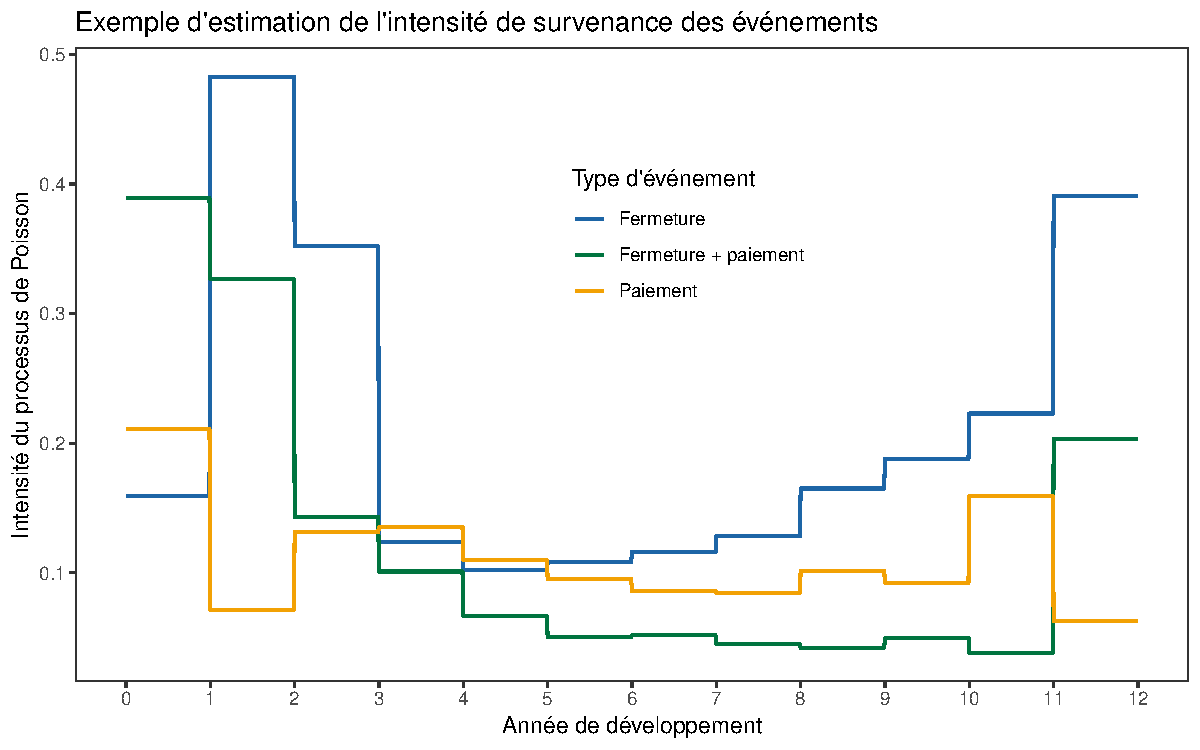
\includegraphics[width = \textwidth]{fonctions_intensite_evenements_janvier_2020.pdf}
    \end{figure}

\end{frame}

% ----------

\begin{frame}{Simulation d'une réclamation RBNS}
    
    \begin{itemize}
        \onslide<2->{\item[\circled{1}] \textbf{Simuler le temps avant le prochain événement.}}
        \onslide<4->{\item[\circled{2}] \textbf{Simuler le type d'événement.}}
        \onslide<6->{
            \item[\circled{3}] \textbf{Selon le type d'événement simulé, choisir l'action à effectuer:}
            \begin{itemize}
                \cercle \alert{Paiement}: simuler le montant du paiement, retourner à \circled{1}.
                \cercle \alert{Paiement $+$ fermeture}: simuler le montant, arrêter la simulation.
                \cercle \alert{Fermeture}: arrêter la simulation.
            \end{itemize}
        }
    \end{itemize}
    
    \begin{figure}
    	\centering
    	\begin{tikzpicture}[scale = 0.8, color = mgris]
    		
    		\onslide<1->{\draw[->, very thick] (0, 0) -- (13.5, 0);}
    		\onslide<1->{\draw[dashed, thick] (7, -1) -- (7, 3);}
    		\onslide<1->{\node at (7, -1.5) {Date};}
    		\onslide<1->{\node at (7, -2) {d'évaluation};}
    		
    		\onslide<1->{\node at (2, 2) {\croixrouge};}
    		\onslide<1->{\draw[dotted, thick] (2.2, 2) -- (6, 2);}
    		\onslide<1->{\node at (6.1, 2) {\trianglevert};}
    		\onslide<1->{\draw[line width = 0.25mm] (6.25, 2) -- (7, 2);}
    		\onslide<3-6>{\draw[line width = 0.25mm, grispale] (7, 2) -- (9.8, 2);}
    		\onslide<5->{\fill[mbleupalepale] (10, 2) circle (0.13);}
    		\onslide<7->{\draw[line width = 0.25mm, grispale] (7, 2) -- (9.6, 2);}
    		\onslide<7->{\fill[mbleupalepale] (10, 2) circle (0.3);}
    		\onslide<8->{\draw[line width = 0.25mm, grispale] (10.4, 2) -- (12, 2);}
    		\onslide<9->{\draw[fill = grispale, color = grispale](12, 1.9) rectangle ++(0.2, 0.2);}
    		
    		\onslide<10->{\node at (1, 1) {\croixrouge};}
    		\onslide<10->{\draw[dotted, thick] (1.2, 1) -- (3, 1);}
    		\onslide<10->{\node at (3.1, 1) {\trianglevert};}
    		\onslide<10->{\draw[line width = 0.25mm] (3.25, 1) -- (5, 1);}
    		\onslide<10->{\fill[mbleupale] (5.2, 1) circle (0.11);}
    		\onslide<10->{\draw[line width = 0.25mm] (5.4, 1) -- (7, 1);}
    		\onslide<11->{\draw[line width = 0.25mm, grispale] (7, 1) -- (8.55, 1);}
    		\onslide<12->{\fill[mbleupalepale] (8.7, 1) circle (0.11);}
    		\onslide<13->{\draw[line width = 0.25mm, grispale] (8.85, 1) -- (10.5, 1);}
    		\onslide<14->{\fill[grispale] (10.5, 1) circle (0.16);}
    		
    		\onslide<1->{\node[anchor = west] at (0, -0.5) {\footnotesize Accident};}
            \onslide<1->{\node[anchor = west] at (0, -0.9) {\footnotesize Déclaration};}
            \onslide<1->{\node[anchor = west] at (0, -1.3) {\footnotesize Paiement};}
            \onslide<1->{\node[anchor = west] at (0, -1.7) {\footnotesize Paiement $+$ Fermeture};}
            \onslide<1->{\node[anchor = west] at (0, -2.1) {\footnotesize Fermeture};}
            
            \onslide<1->{\node at (-0.1, -0.5) {\croixrouge};}
            \onslide<1->{\node at (-0.1, -0.9) {\trianglevert};}
            \onslide<1->{\fill[mbleupalepale] (-0.1, -1.3) circle (0.13);}
            \onslide<1->{\fill[grispale] (-0.1, -1.7) circle (0.13);}
            \onslide<1->{\draw[fill = grispale, color = grispale](-0.195, -2.2) rectangle ++(0.2, 0.2);}
    		
    	\end{tikzpicture}
    \end{figure}

\end{frame}


% ----------

\begin{frame}{Simulation d'une réclamation IBNR}

    \begin{itemize}
        \onslide<1->{\item[\circled{1}] \textbf{Simuler la survenance de la réclamation.}}
        \onslide<3->{\item[\circled{2}] \textbf{Simuler le délai de déclaration, sachant que la déclaration est postérieure à la date d'évaluation.}}
        \onslide<5->{\item[\circled{3}] \textbf{Simuler le processus de développement de la même manière qu'une réclamation RBNS.}}
    \end{itemize}
    
    
    \begin{figure}
    	\centering
    	\begin{tikzpicture}[scale = 0.8, color = mgris]
    		
    		\draw[->, very thick] (0, 0) -- (13.5, 0);
    		\draw[dashed, thick] (7, -1) -- (7, 3);
    		\node at (7, -1.5) {Date};
    		\node at (7, -2) {d'évaluation};
    		
    		\onslide<2->{\node at (5, 2) {\croixrouge};}
    		\onslide<4->{\draw[dotted, thick, grispale] (5.2, 2) -- (8.1, 2);}
    		\onslide<4->{\node at (8.2, 2) {\trianglevert};}
    		\onslide<6->{\draw[line width = 0.25mm, grispale] (8.3, 2) -- (9, 2);}
    		\onslide<6->{\fill[mbleupalepale] (9.2, 2) circle (0.17);}
    		\onslide<6->{\draw[line width = 0.25mm, grispale] (9.4, 2) -- (11, 2);}
    		\onslide<6->{\fill[mbleupalepale] (11.2, 2) circle (0.17);}
    		\onslide<6->{\draw[line width = 0.25mm, grispale] (11.4, 2) -- (12, 2);}
    		\onslide<6->{\draw[fill = grispale, color = grispale](12, 1.9) rectangle ++(0.2, 0.2);}
    		
    		\onslide<2->{\node at (3.5, 1) {\croixrouge};}
    		\onslide<4->{\draw[dotted, thick, grispale] (3.7, 1) -- (8.9, 1);}
    		\onslide<4->{\node at (9.1, 1) {\trianglevert};}
    		\onslide<6->{\draw[line width = 0.25mm, grispale] (9.25, 1) -- (11, 1);}
    		\onslide<6->{\fill[grispale] (11, 1) circle (0.19);}
    		
    		\node[anchor = west] at (0, -0.5) {\footnotesize Accident};
            \node[anchor = west] at (0, -0.9) {\footnotesize Déclaration};
            \node[anchor = west] at (0, -1.3) {\footnotesize Paiement};
            \node[anchor = west] at (0, -1.7) {\footnotesize Paiement $+$ Fermeture};
            \node[anchor = west] at (0, -2.1) {\footnotesize Fermeture};
            
            \node at (-0.1, -0.5) {\croixrouge};
            \node at (-0.1, -0.9) {\trianglevert};
            \fill[mbleupalepale] (-0.1, -1.3) circle (0.13);
            \fill[grispale] (-0.1, -1.7) circle (0.13);
            \draw[fill = grispale, color = grispale](-0.195, -2.2) rectangle ++(0.2, 0.2);
    		
    	\end{tikzpicture}
    \end{figure}
    
\end{frame}

% ----------

\begin{frame}{Détermination de la réserve}
    
    \begin{itemize}
        \fleche \textbf{RBNS}
            \begin{itemize}
                \cercle Simuler le processus de développement de toutes les réclamations RBNS du portefeuille.
            \end{itemize}
        
        \fleche \textbf{IBNR}
            \begin{itemize}
                \cercle Simuler la survenance des réclamations IBNR.
                \cercle Simuler le délai de déclaration des réclamations IBNR.
                \cercle Simuler le processus de développement des réclamations IBNR.
            \end{itemize}
        \fleche \textbf{Réserve simulée = somme des paiements simulés}
        \fleche \textbf{Plusieurs simulations pour obtenir la distribution prédictive.}
    \end{itemize}
    
    \begin{alertblock}{Note}
        Pour les réclamations IBNR, il faut simuler les variables explicatives puisqu'elles ne sont pas observées à la date d'évaluation.
    \end{alertblock}
    
\end{frame}

% ----------

\section{Adaptation à la base de données simulée}

% ----------

\begin{frame}{Simulation des données de réclamations}

    \begin{itemize}[itemsep = 0.25cm]
        \fleche Données simulées avec \texttt{Gabrielli, A., \& Wüthrich, M. (2018). An individual claims history simulation machine. \emph{Risks, 6}(2).}
        \fleche Plusieurs réseaux de neurones entrainés sur des données réelles.
        \fleche Le délai de déclaration et le processus de développement dépendent de 6 caractéristiques de la réclamation (\texttt{ligne d'affaire}, \texttt{code de réclamation}, \texttt{année d'accident}, \texttt{trimestre d'accident}, \texttt{âge}, \texttt{partie du corps blessée}).
        \fleche Simulation en temps discret.
    \end{itemize}
    
\end{frame}

% ----------

\begin{frame}{Simulation des données de réclamations}

    \textbf{Extrait de la base de données simulée}:

    \resizebox{\textwidth}{!}{
    \begin{table}[h]
        \centering
        \begin{tabular}{c|cccccc|c|ccccc|ccccc}
            \toprule
            \midrule
            \textbf{Claim #} & \textbf{LoB} & \textbf{cc} & \textbf{AY} & \textbf{AQ} & \textbf{age} & \textbf{inj\_part} & \textbf{RepDel} & \textbf{Pay00} & \textbf{Pay01} & \textbf{Pay02} & \textbf{\dots} & \textbf{Pay11} & \textbf{Open00} & \textbf{Open01} & \textbf{Open02} & \textbf{\dots} & \textbf{Open11}\\
            \midrule
            \rowcolor{gray!15} 1 & 3 & 17 & 94 & 2 & 23 & 11 & 0 & 0 & 0 & 0 & \dots & 0 & 0 & 0 & 0 & \dots & 0\\
            2 & 4 & 19 & 94 & 3 & 32 & 21 & 0 & 113 & 0 & 0 & \dots & 0 & 1 & 0 & 0 & \dots & 0\\
            \rowcolor{gray!15} 3 & 4 & 39 & 94 & 2 & 47 & 10 & 0 & 180 & 0 & 0 & \dots & 0 & 0 & 0 & 0 & \dots & 0\\
            4 & 3 & 27 & 94 & 4 & 35 & 51 & 0 & 0 & 2582 & 0 & \dots & 0 & 1 & 0 & 0 & \dots & 0\\
            \rowcolor{gray!15} 5 & 2 & 29 & 94 & 1 & 15 & 61 & 0 & 0 & 1656 & 0 & \dots & 0 & 1 & 0 & 0 & \dots & 0\\
            6 & 2 & 9 & 94 & 2 & 63 & 53 & 0 & 3094 & 0 & 0 & \dots & 0 & 0 & 0 & 0 & \dots & 0\\
            \rowcolor{gray!15} 7 & 4 & 42 & 94 & 1 & 41 & 21 & 0 & 631 & 0 & 0 & \dots & 0 & 0 & 0 & 0 & \dots & 0\\
            8 & 2 & 43 & 94 & 3 & 35 & 52 & 0 & 0 & 2059 & 0 & \dots & 0 & 1 & 0 & 0 & \dots & 0\\
            \rowcolor{gray!15} 9 & 2 & 34 & 94 & 1 & 45 & 10 & 0 & 0 & 0 & 0 & \dots & 0 & 0 & 0 & 0 & \dots & 0\\
            10 & 2 & 1 & 94 & 4 & 37 & 34 & 0 & 0 & 1039 & 0 & \dots & 0 & 1 & 0 & 0 & \dots & 0\\
            \hline
            \bottomrule
        \end{tabular}
    \end{table}
    }

\end{frame}

% ----------

\begin{frame}{Adaptation du modèle aux données simulées}

    \begin{itemize}
        \fleche \textbf{Modifications faites au modèle}
        \begin{itemize}
            \cercle On peut voir les données discrètes comme des données continues qui, miraculeusement, ressemblent à des données discrètes.
            \cercle Seul problème: le délai de déclaration, modélisé par une loi Weibull.
            \cercle On remplace donc la Weibull par n'importe quelle loi discrète (j'ai utilisé une binomiale négative).
            \cercle Le modèle est entrainé sur des données discrètes, mais simule des données continues.
        \end{itemize}
        \vspace{0.5cm}
        \fleche \textbf{Modifications faites à la base de données simulée}
        \begin{itemize}
            \cercle Suppression des paiements négatifs.
            \cercle Ignorance des réouvertures.
            \cercle Autres modifications mineures.
        \end{itemize}

    \end{itemize}
    
\end{frame}

% ----------

\begin{frame}{Résultats sur données simulées}

    \begin{figure}
        \centering
        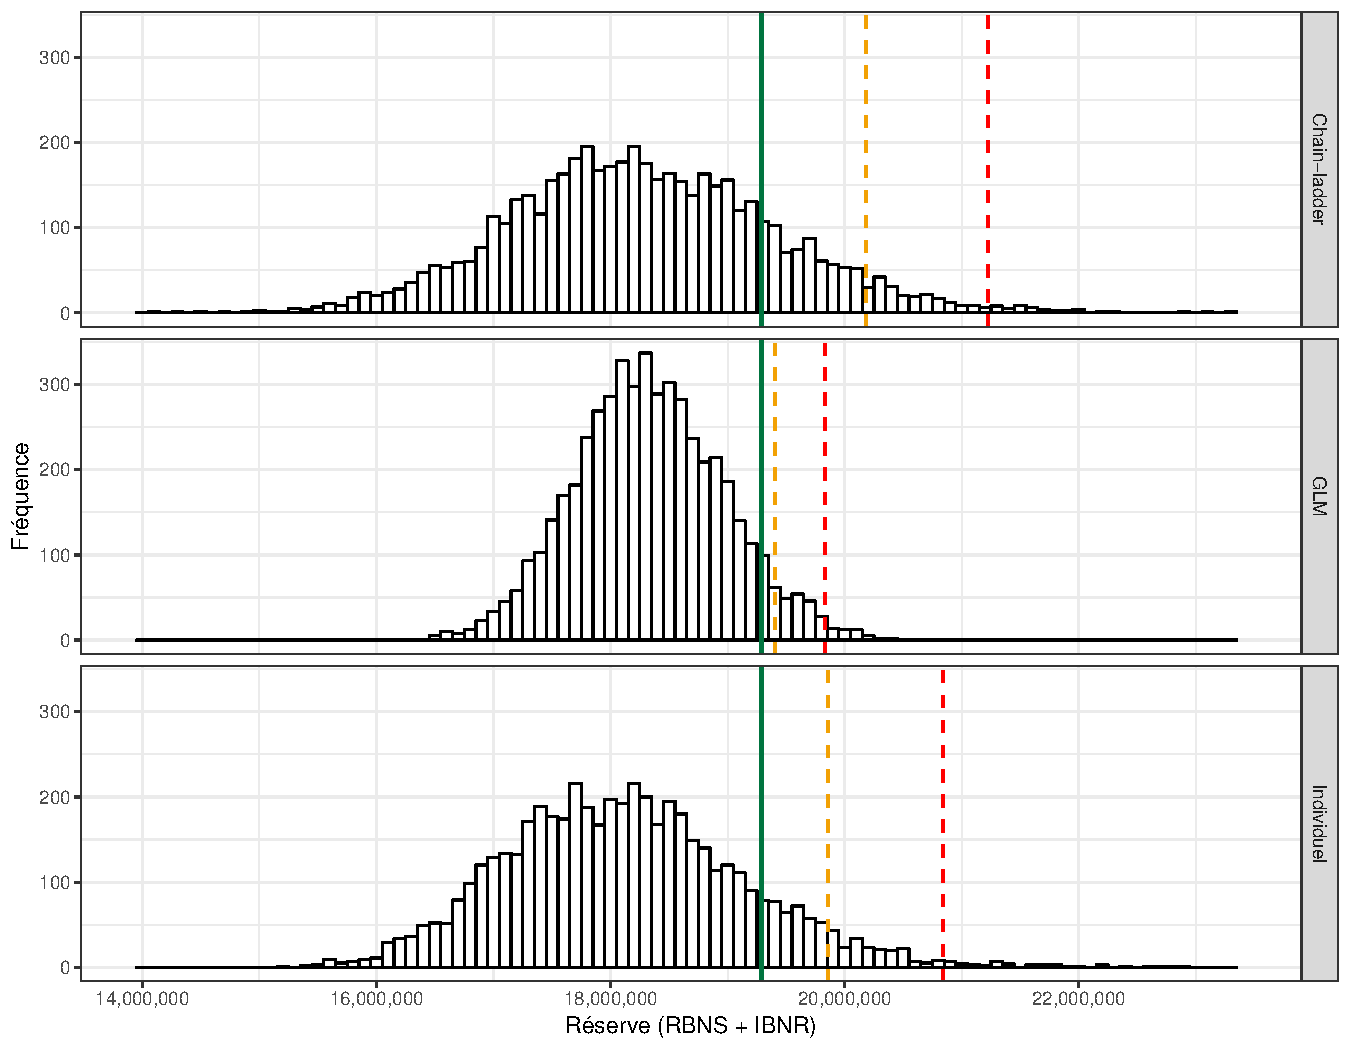
\includegraphics[width = 0.85\textwidth]{comparaison_ind_coll_2.pdf}
    \end{figure}

\end{frame}

% ----------

\section{Modifications -- Francis}

% ----------

\begin{frame}{Mise en contexte}

    \begin{exampleblock}{Question guide}
        La régression quantile permet-elle de mieux modéliser la sévérité des paiements que les GLM en provisionnement non-vie?
    \end{exampleblock}
    
    \begin{alertblock}{Résumé du projet}
        \begin{itemize}
            \fleche Modélisation de la sévérité des paiements avec la régression quantile.
        \end{itemize}
    \end{alertblock}

\end{frame}

% ----------

\begin{frame}{Mise en contexte}

    \begin{itemize}[itemsep = 0.4cm]
        \fleche Variable réponse: log-paiement.
        \fleche Variable explicative: année de développement.
        \fleche Ensemble d'entrainement: contient tous les paiements observés avant 2006 (79 921 observations).
        \fleche Ensemble de validation: contient tous les paiements associés au réclamations RBNS observés après 2006 (3153 observations).
    \end{itemize}
    \vspace{0.8cm}
    \begin{tikzpicture}[scale = 0.7, rotLabel/.style = {above = 3pt, rotate = 90, anchor = 200, right = 3pt}]
    	% Fleche ligne du temps
    	\draw[->, very thick] (0, 0) -- (15, 0);
    	% Années
    	\draw (1, 0) node[below = 3pt] {1994};
    	\draw (8, 0) node[below = 3pt] {2006};
    	% Ticks
    	\foreach \x in {1, 8}
          	\draw (\x cm,3pt) -- (\x cm, -3pt);
    	% Curly braces
    	\draw [thick, decorate, decoration = {brace, amplitude = 5pt, raise = 4pt}] (1.05, 0) -- (7.95, 0);
    	\draw [thick, decorate, decoration = {brace, amplitude = 5pt, raise = 4pt}] (8.05, 0) -- (14.7, 0);
    	% Écriture
    	\draw (4.5, 0) node[above = 10pt] {Entrainement};
    	\draw (11.35, 0) node[above = 10pt] {Validation};
    \end{tikzpicture}
    
\end{frame}

% ----------

\begin{frame}{Régression quantile}

\begin{exampleblock}{Régression linéaire}
    
\end{exampleblock}
    
\end{frame}

% ----------

\begin{frame}{Nombre de quantiles comme hyperparamètre}

\begin{itemize}[itemsep = 0.4cm]
    \fleche Traiter le nombre de quantiles modélisés comme un hyperparamètre.
    \begin{itemize}
        \blt Pas assez de quantiles: sous-ajustement
        \blt Trop de quantiles: surajustement
    \end{itemize}
    \fleche \textit{Machine learning}: hyperparamètres déterminés en calculant une distance entre l'observé et la prédiction \alert{ponctuelle} (RMSE, MAE, etc.) sur échantillon test (ou avec validation croisée). 
    \fleche Dans le cadre des réserves individuelles, on veut mesurer la distance entre la \alert{distribution} observée et prédite.
    \fleche On a donc besoin d'une statistique qui mesure la distance entre 2 distributions.
\end{itemize}
    
\end{frame}

% ----------

\begin{frame}{Statistique de Kolmogorov-Smirnov}

\begin{itemize}
    \fleche Mesure de distance entre 2 distributions.
    \fleche $\text{K-S} = \max_x \left|F_1(x) - F_2(x)\right|$
\end{itemize}
\begin{figure}
    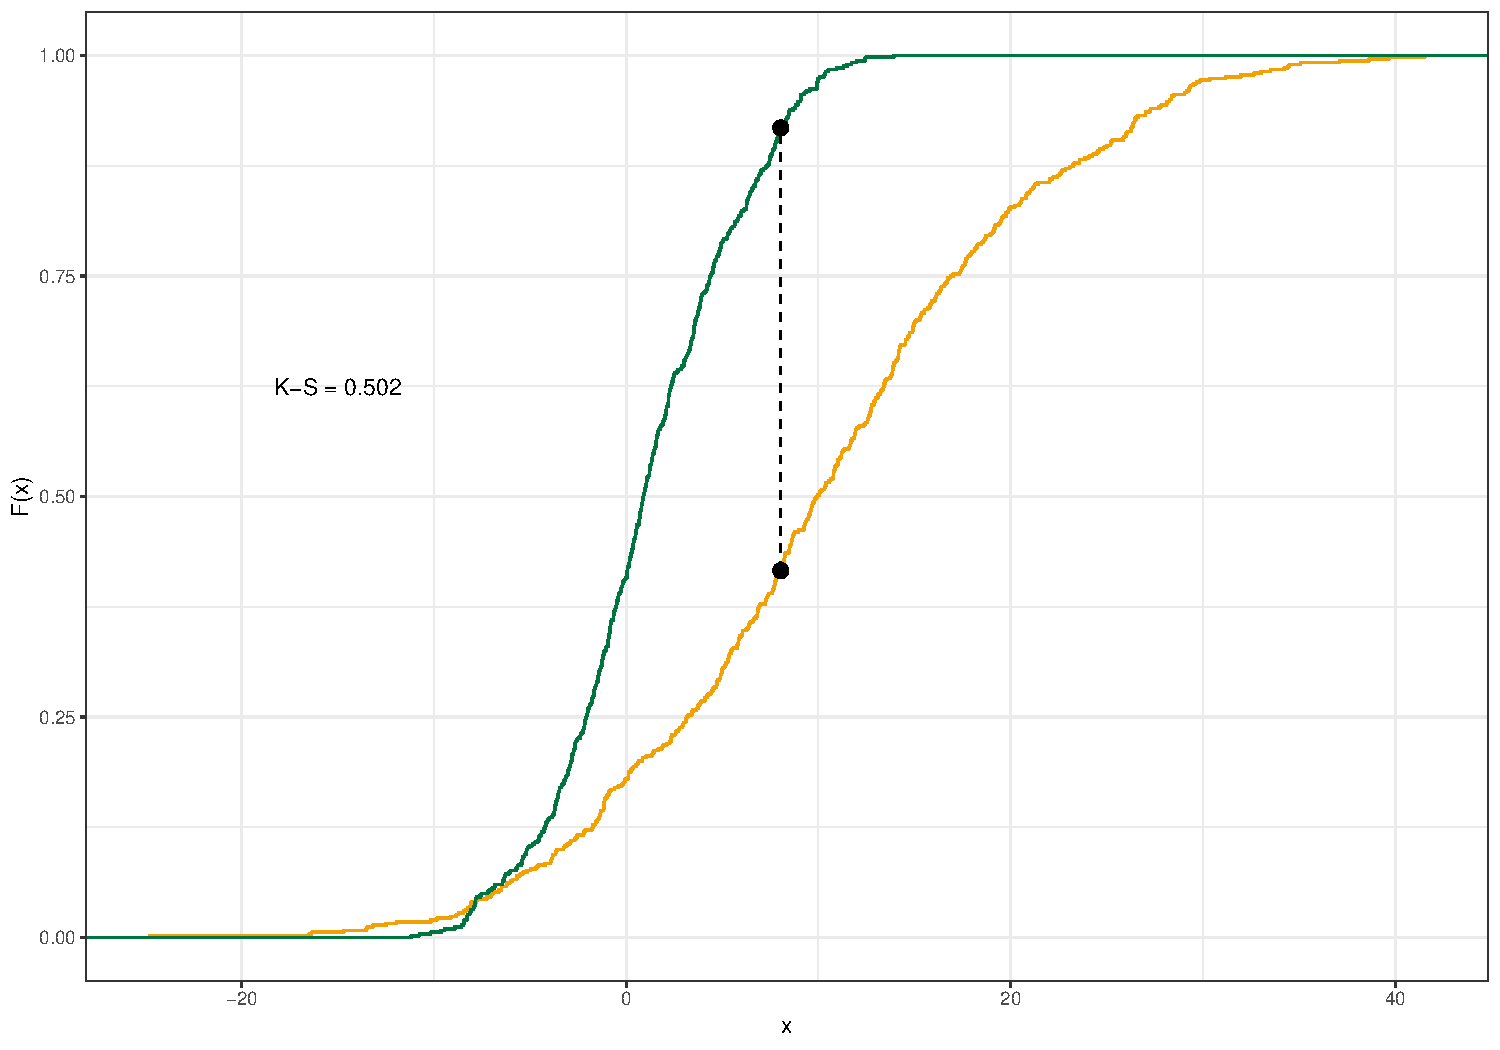
\includegraphics[width = 0.85\textwidth]{ks_plot.pdf}
\end{figure}

\end{frame}

% ----------

\begin{frame}{Procédure pour choisir le nombre de quantiles optimal}
    
\begin{exampleblock}{Procédure}
    \begin{itemize}
        \item[\circled{1}] Séparer l'ensemble d'entrainement en 2: train1 et train2.
        \item[\circled{2}] Ajuster une régression quantile à $n$ quantiles sur train1.
        \item[\circled{3}] À l'aide du modèle ajusté, simuler plusieurs réponses (paiements) pour chaque observation de train2.
        \item[\circled{4}] Calculer la statistique de K-S entre la distribution simulée et la distribution empirique des paiements de train2.
        \item[\circled{5}] Refaire pour plusieurs valeurs de $n$ et choisir $n$ tel que la statistique de K-S est la plus petite.
    \end{itemize}
\end{exampleblock}
    
\end{frame}

% ----------

\begin{frame}{Résultats}

\begin{figure}
    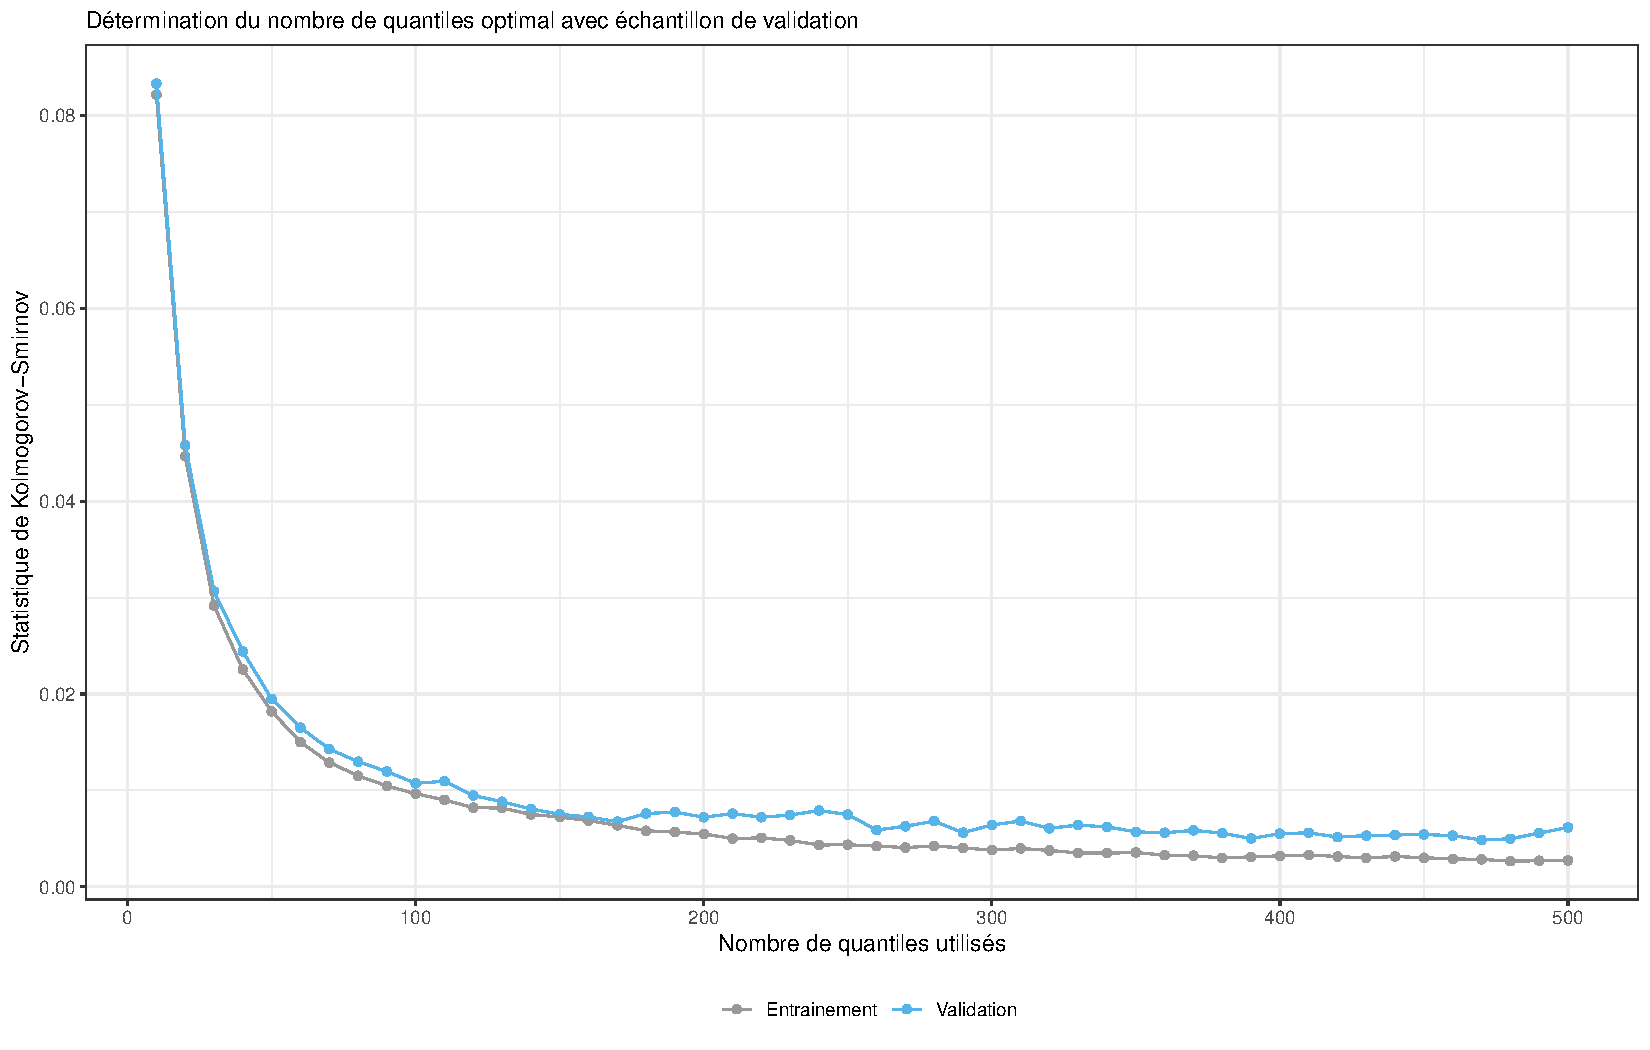
\includegraphics[width = \textwidth]{rq_tuning.pdf}
\end{figure}
    
\end{frame}

% ----------

\begin{frame}{Analyse comparative}

\begin{itemize}[itemsep = 0.4cm]
    \fleche Comparaison de la performance entre la \alert{régression linéaire} et la \alert{régression quantile} sur le jeu de données simulé.
    \fleche Performance mesurée avec la statistique de \alert{Kolmogorov-Smirnov} et avec l'\alert{erreur absolue moyenne} sur le total des paiements.
    \fleche 2 formules considérées: 
    \begin{itemize}
        \blt Modèle linéaire: \texttt{Log-paiement $\sim$ DY}
        \blt Modèle quadratique: \texttt{Log-paiement $\sim$ DY + DY$^2$}
    \end{itemize}
\end{itemize}
    
\end{frame}

% ----------

\begin{frame}{Données d'entrainement et de validation}

\begin{figure}
    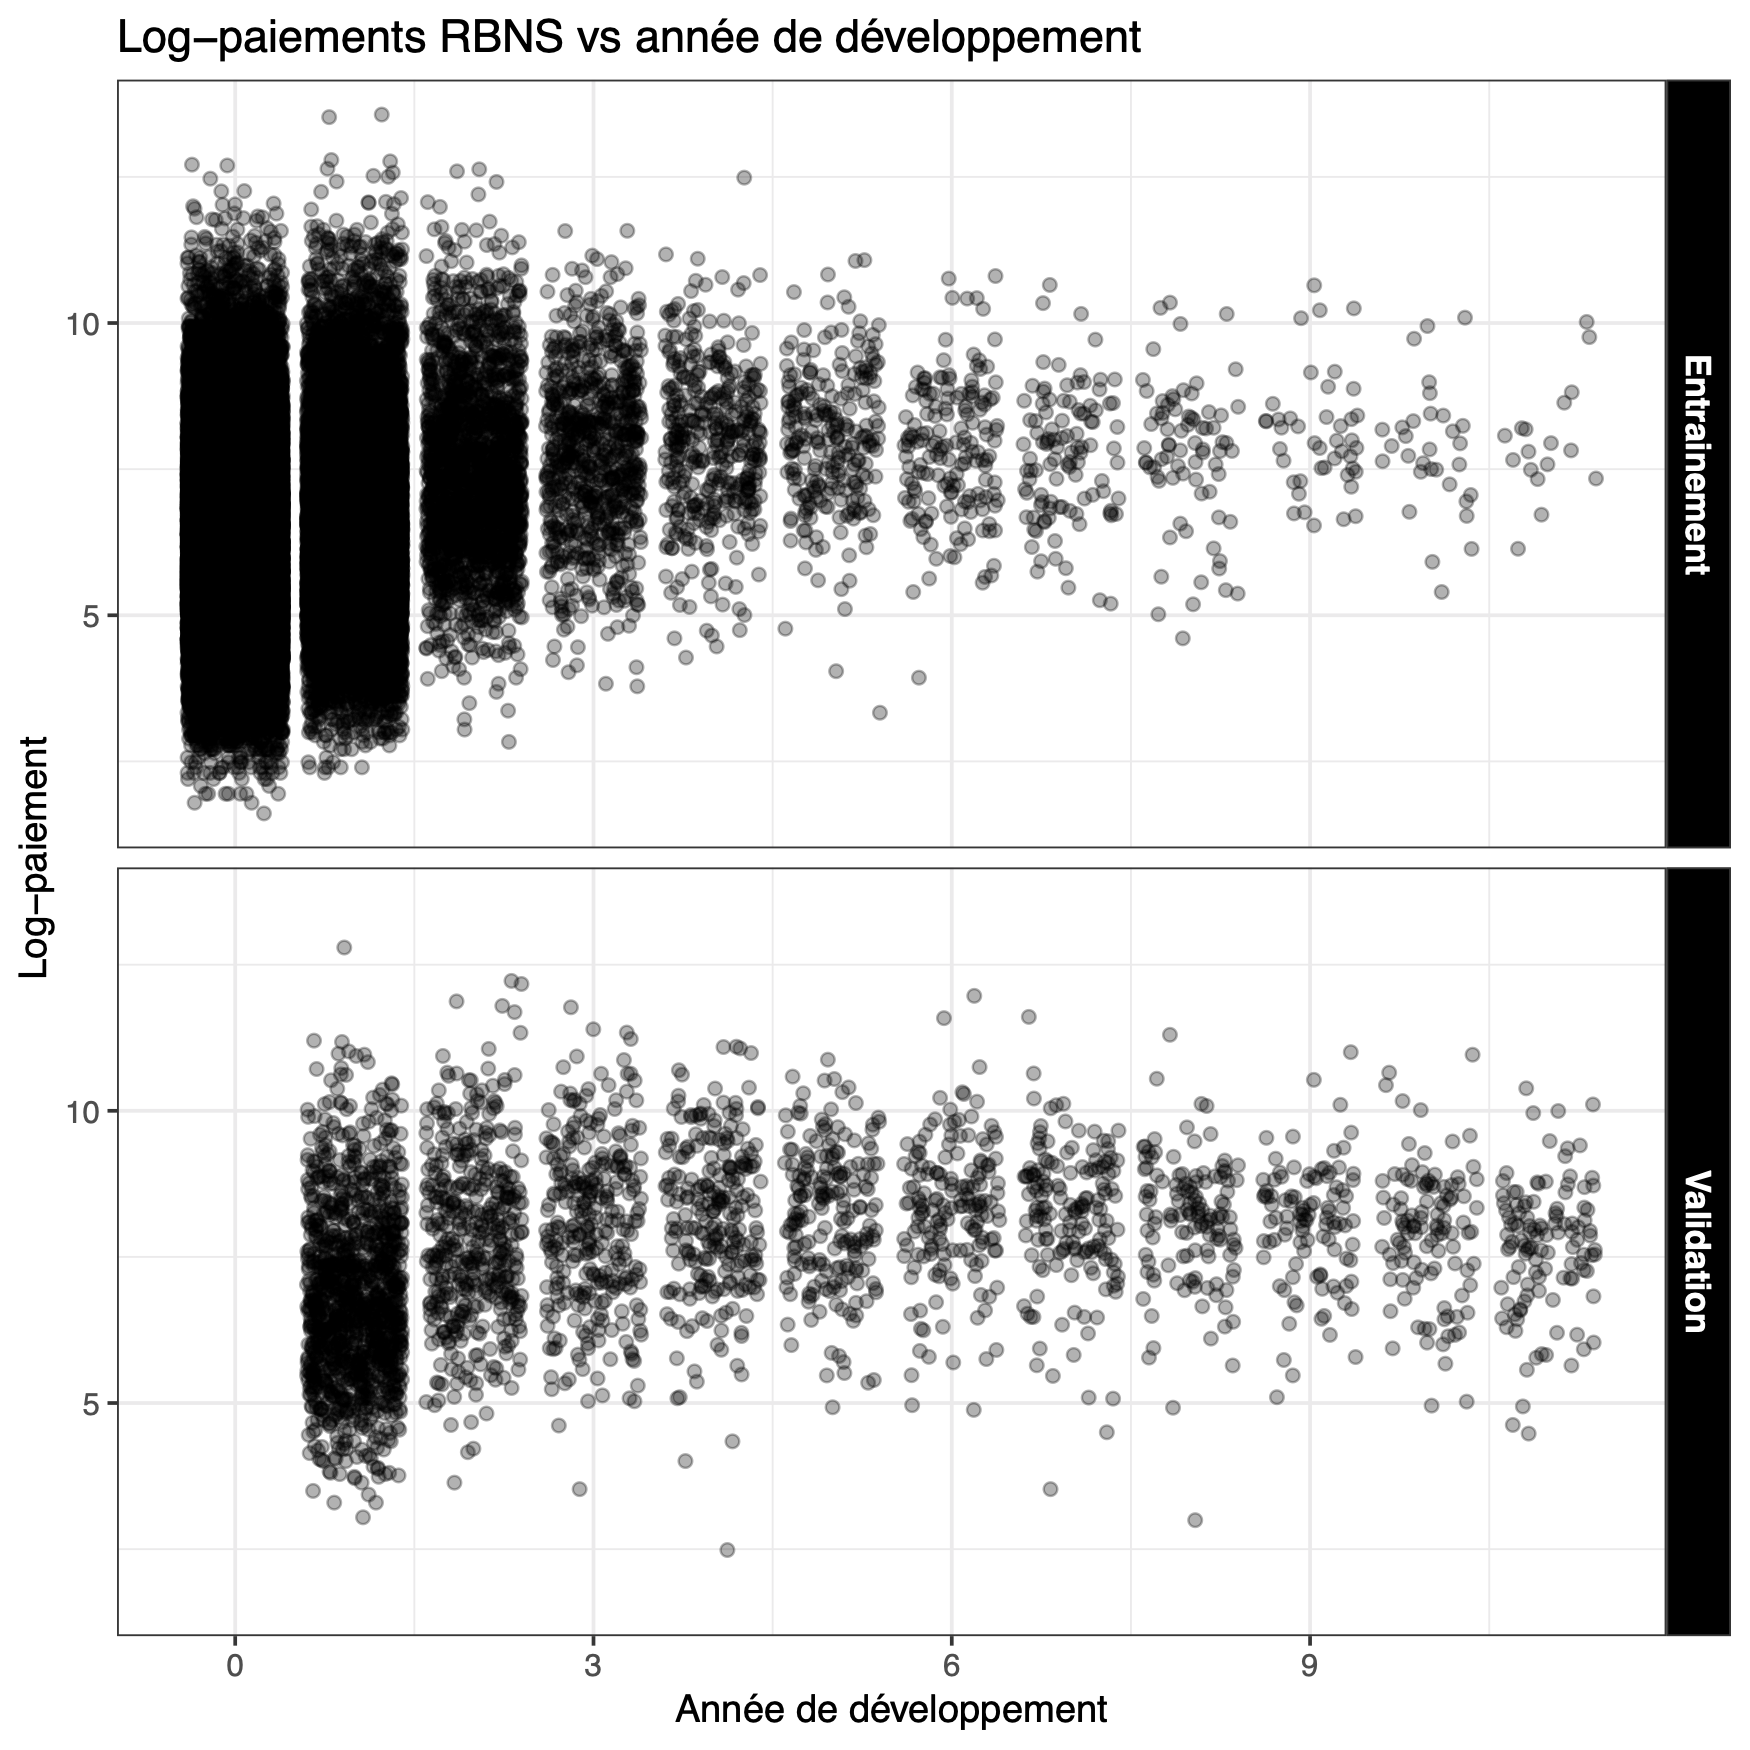
\includegraphics[width = 0.7\textwidth]{train_val_01.png}
\end{figure}
    
\end{frame}

% ----------

\begin{frame}{Entrainement des modèles linéaires}

\begin{figure}
    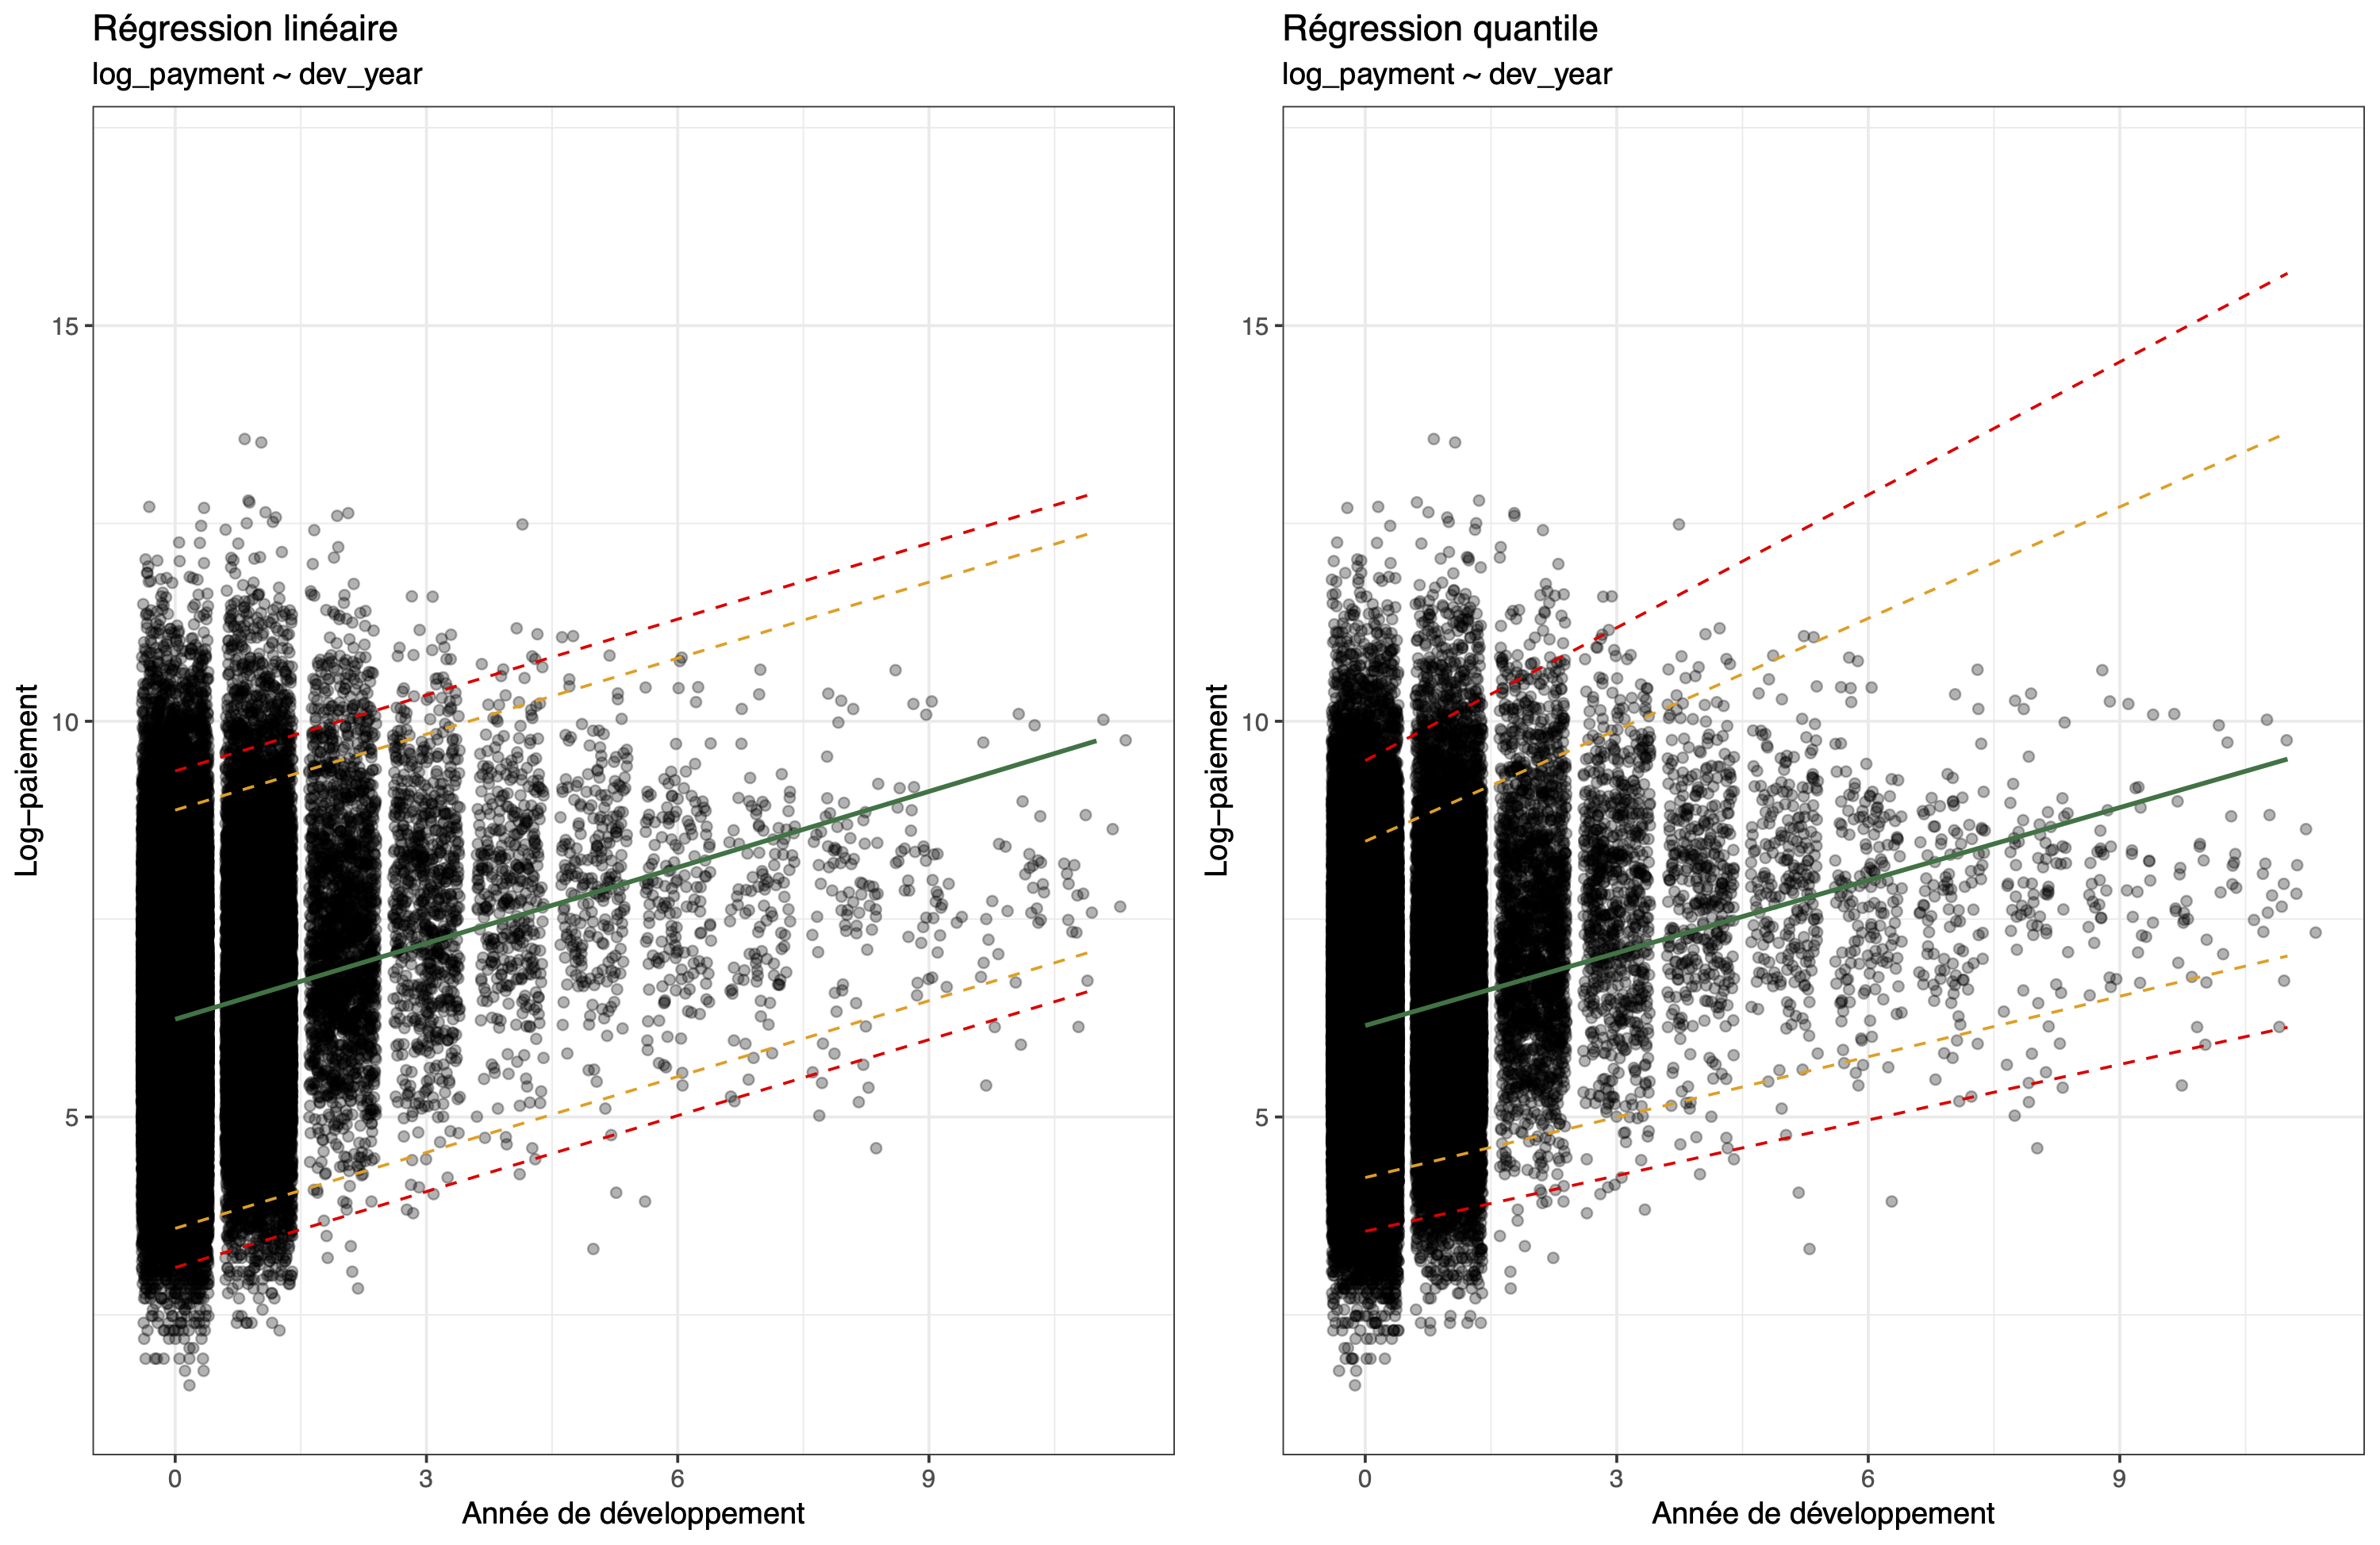
\includegraphics[width = \textwidth]{plot_fit_1.png}
\end{figure}
    
\end{frame}

% ----------

\begin{frame}{Entrainement des modèles quadratiques}

\begin{figure}
    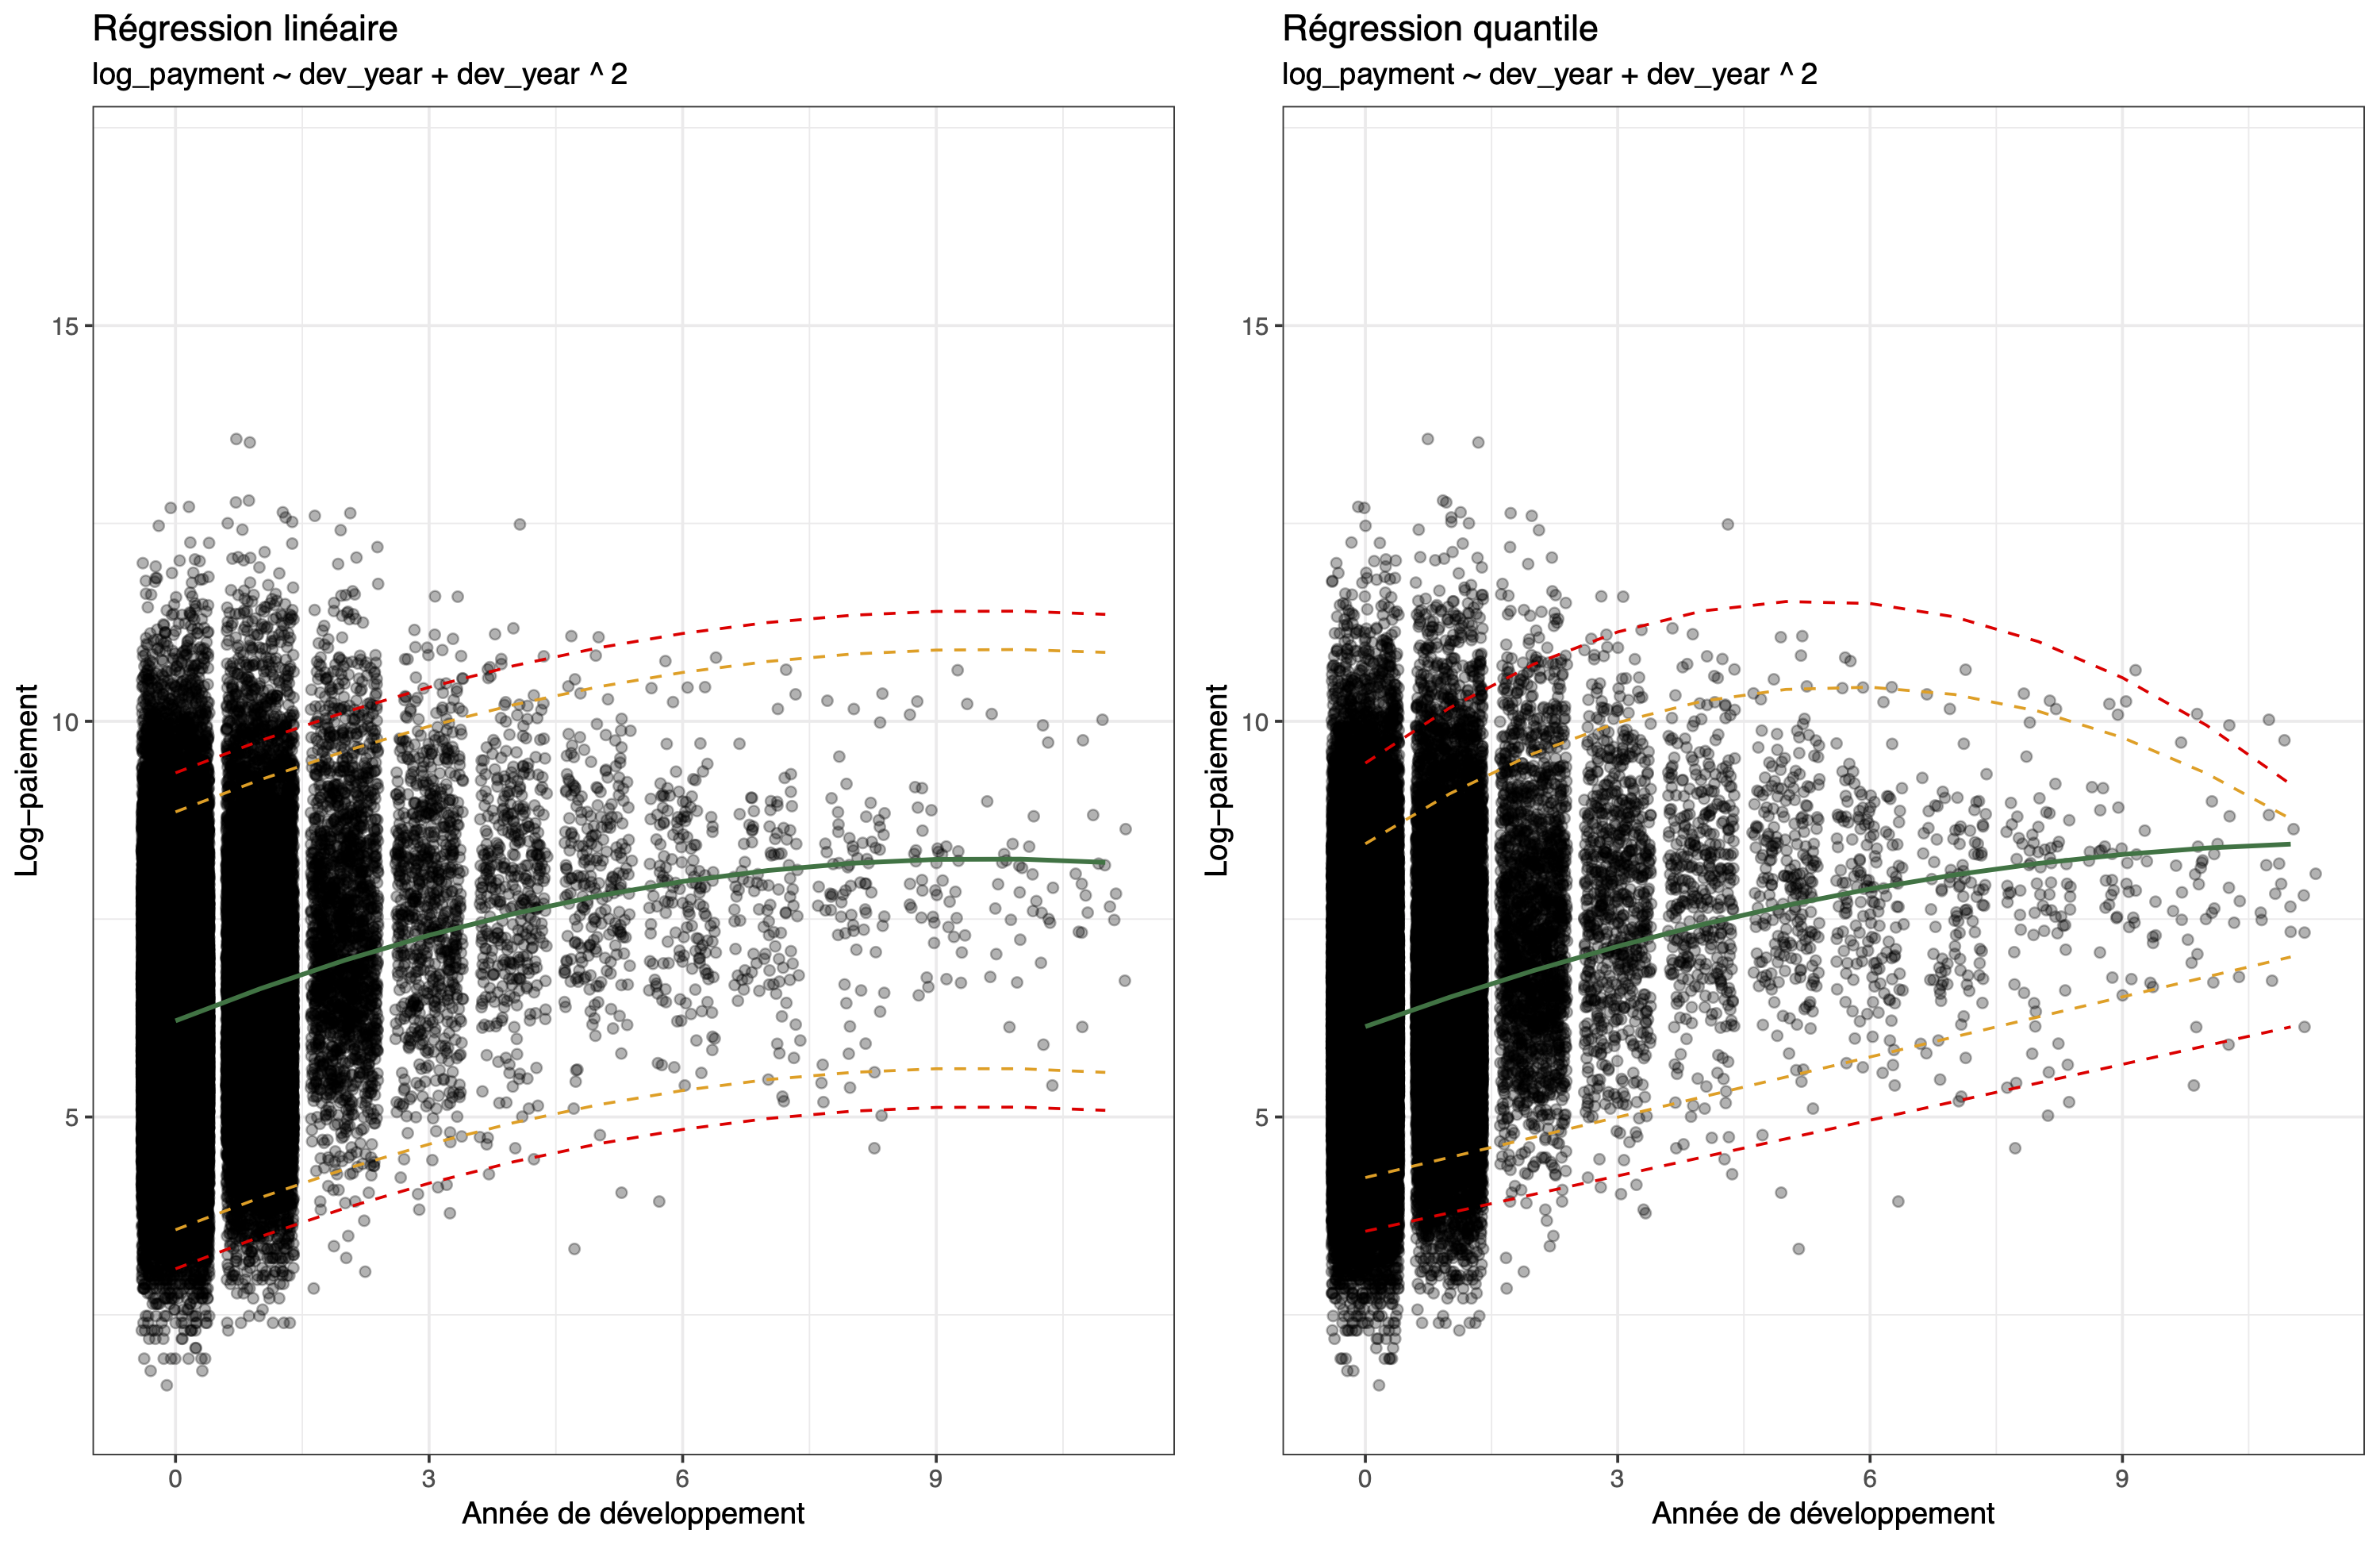
\includegraphics[width = \textwidth]{plot_fit_2.png}
\end{figure}
    
\end{frame}

% ----------

\begin{frame}{Validation des modèles linéaires}

\begin{figure}
    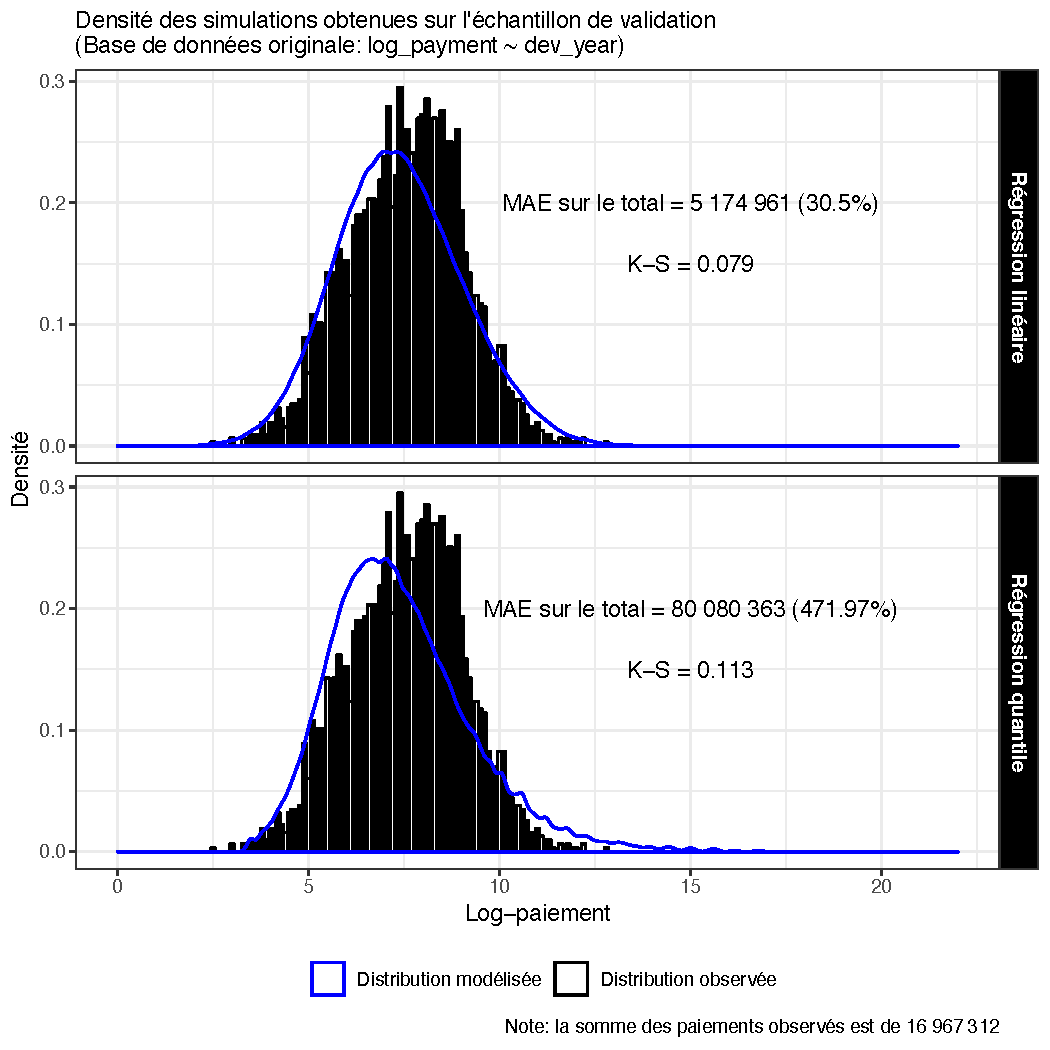
\includegraphics[width = 0.72\textwidth]{plots_valid_1.pdf}
\end{figure}

\end{frame}

% ----------

\begin{frame}{Validation des modèles quadratiques}

\begin{figure}
    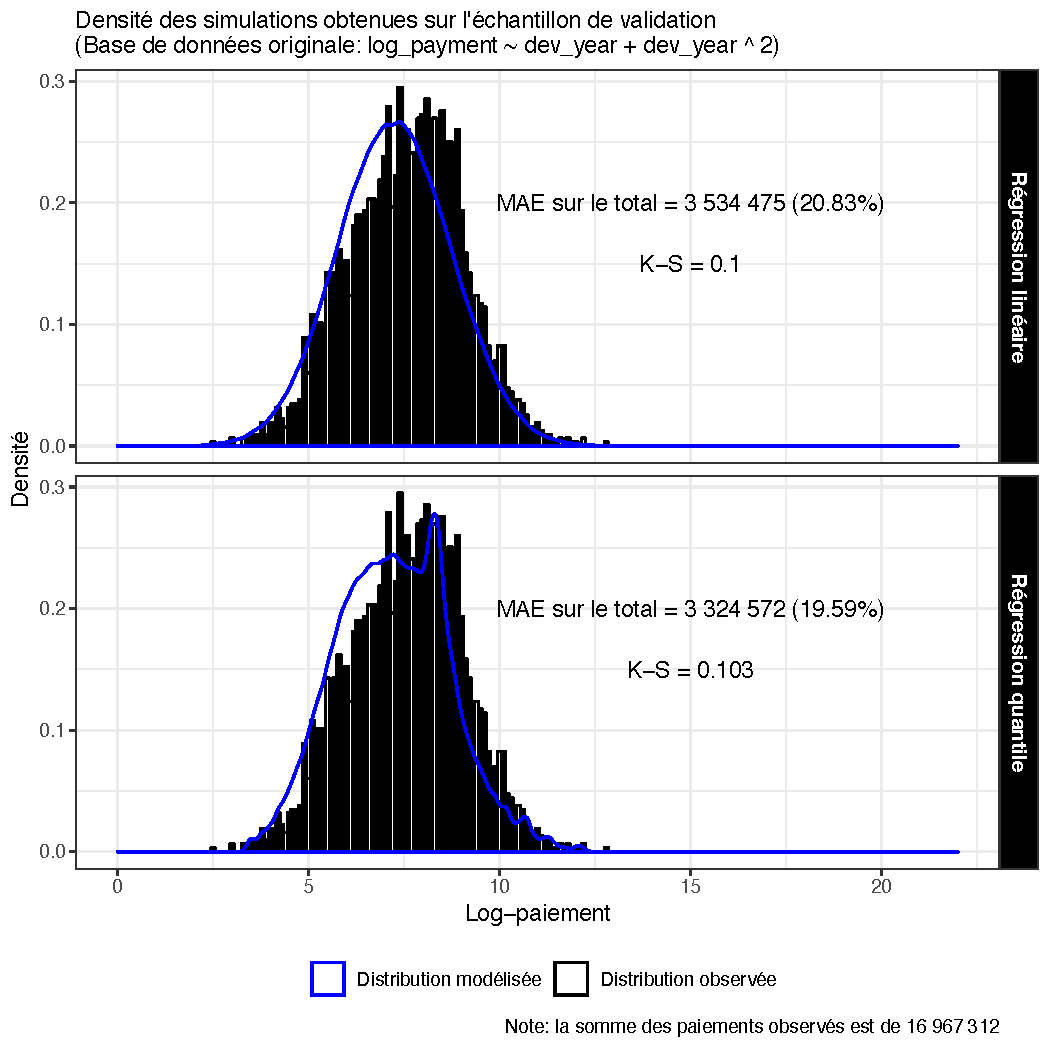
\includegraphics[width = 0.72\textwidth]{plots_valid_2.pdf}
\end{figure}

\end{frame}

% ----------

\begin{frame}{Données d'entrainement et de validation}

\begin{itemize}
    \fleche 5\% des observations ont été prises au hasard et on multiplie la valeur du paiement par 1000.
\end{itemize}

\begin{figure}
    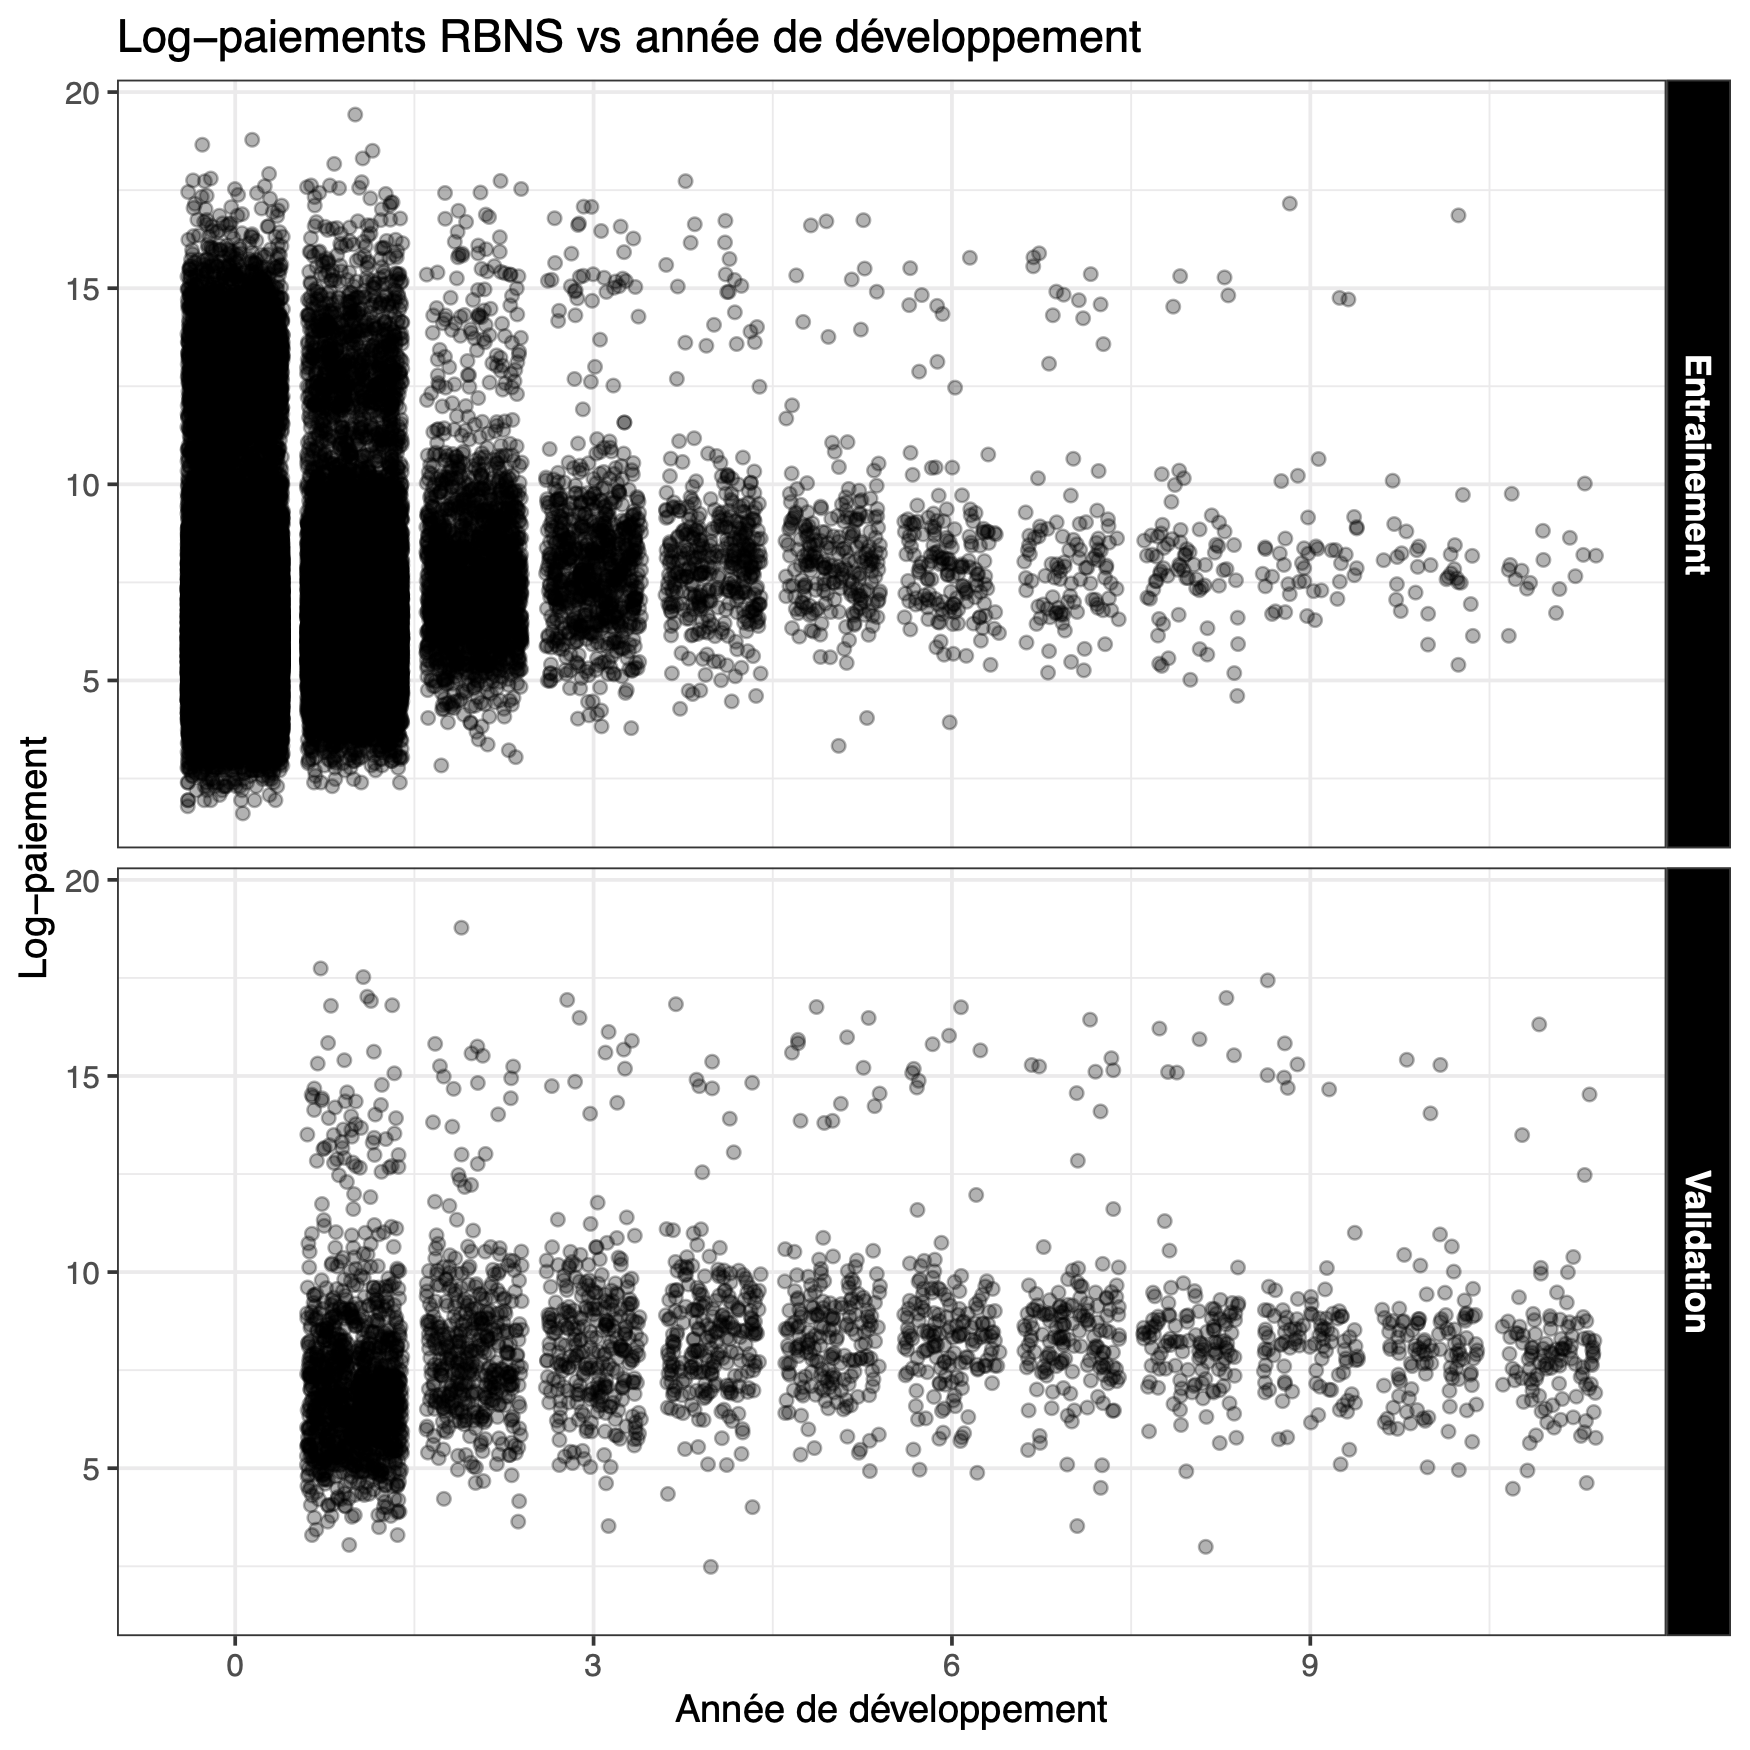
\includegraphics[width = 0.6\textwidth]{train_val_02.png}
\end{figure}

\end{frame}

% ----------

\begin{frame}{Entrainement des modèles quadratiques}

\begin{figure}
    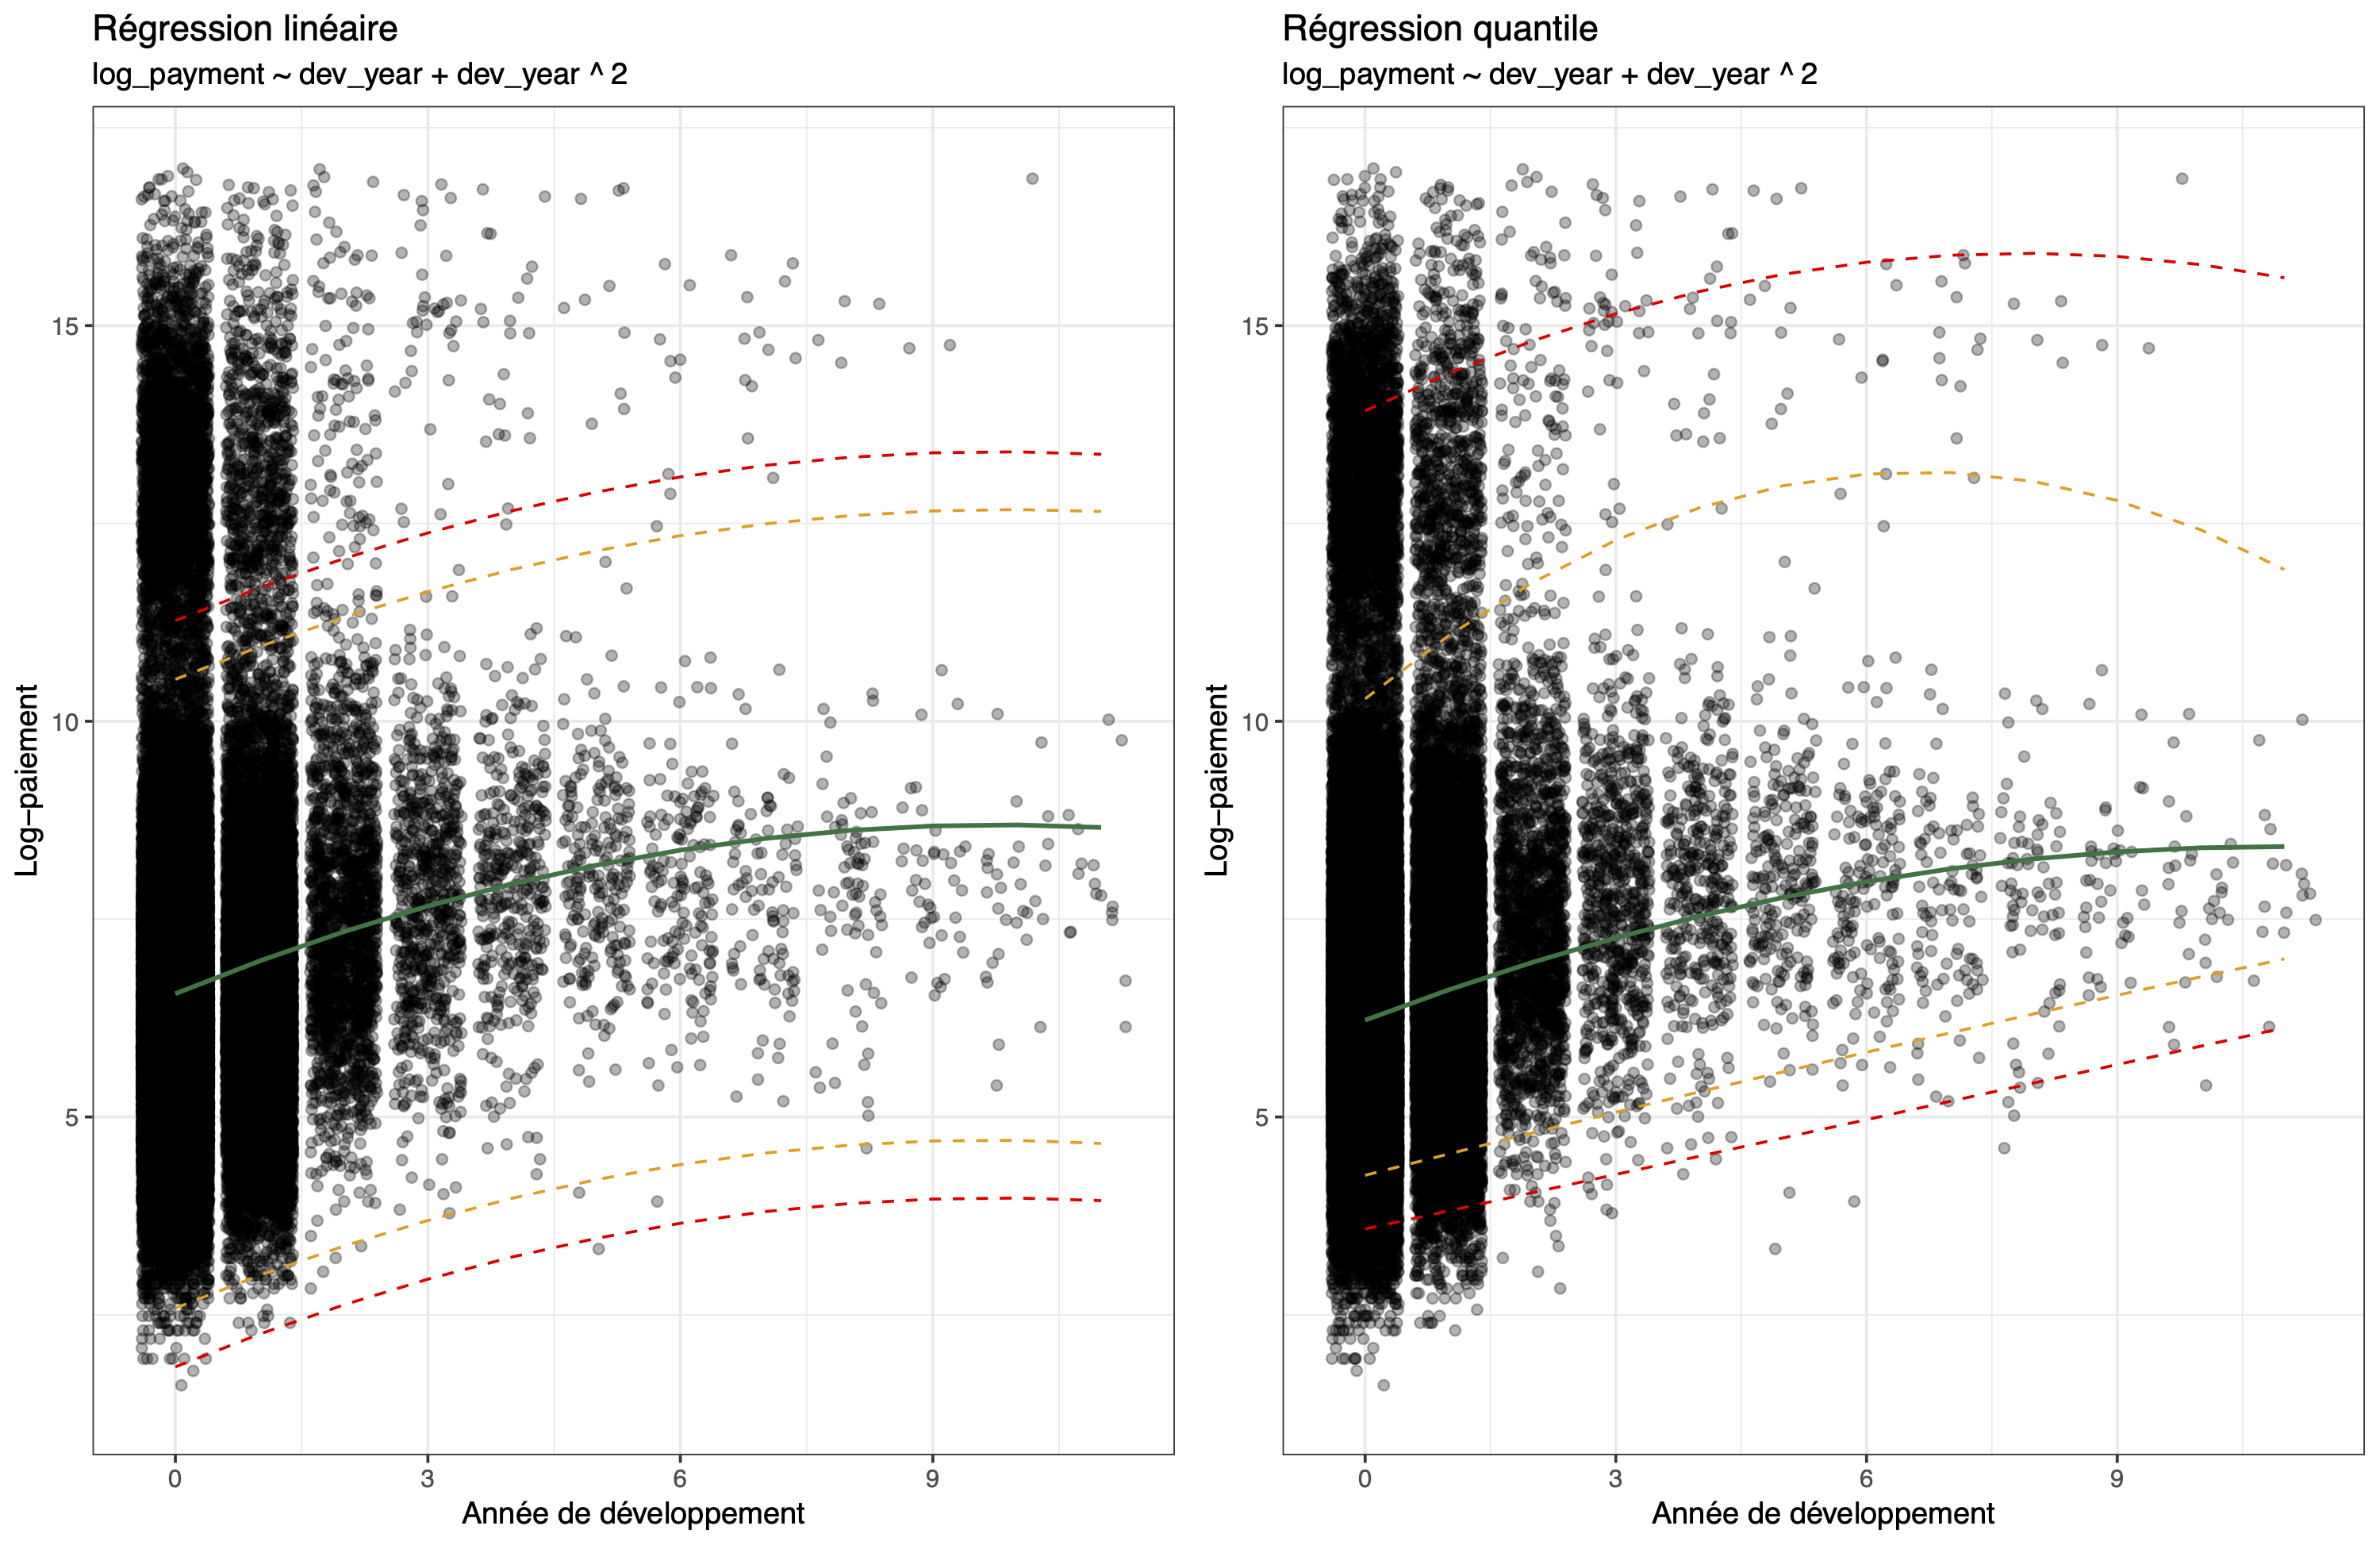
\includegraphics[width = \textwidth]{plot_fit_2_ab.png}
\end{figure}

\end{frame}

% ----------

\begin{frame}{Validation des modèles quadratiques}

\begin{figure}
    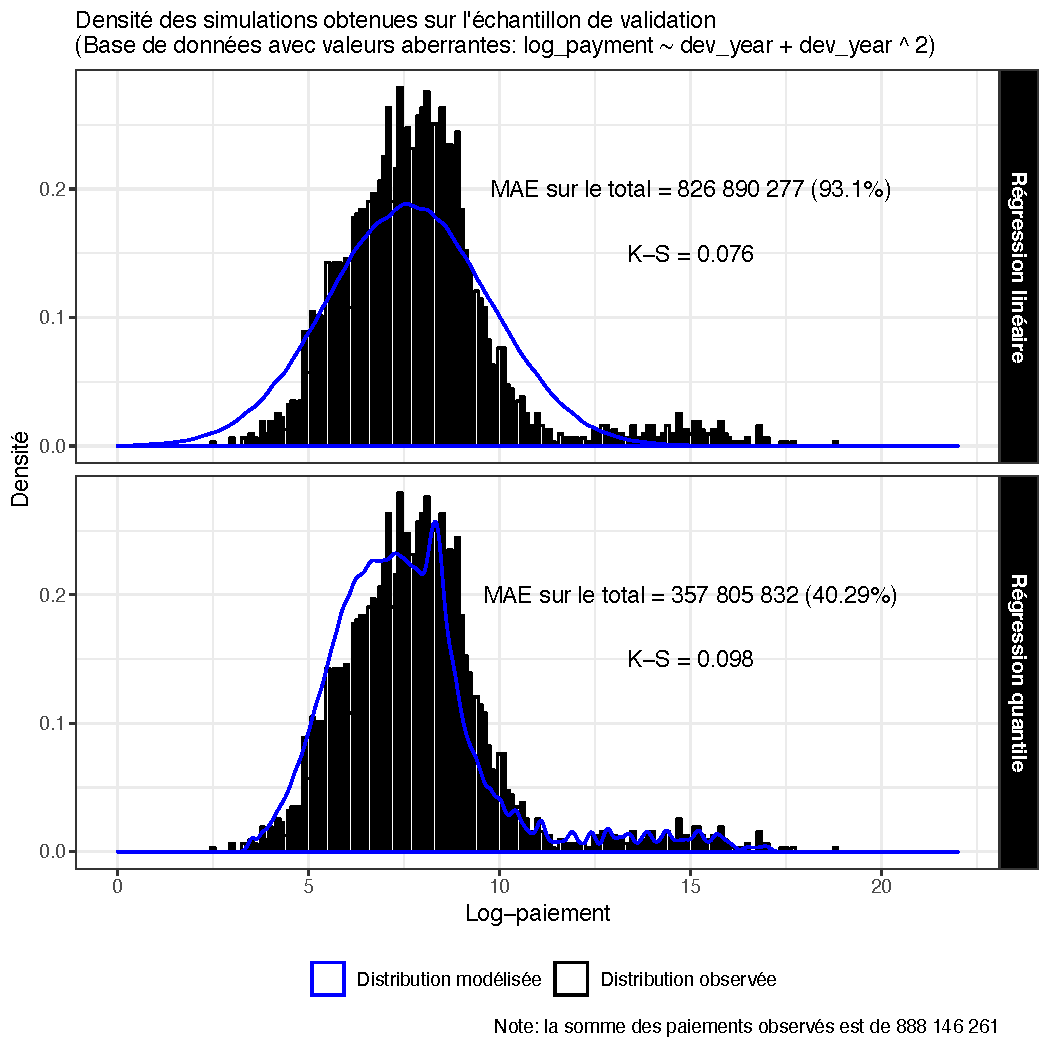
\includegraphics[width = 0.72\textwidth]{plots_valid_2_ab.pdf}
\end{figure}

\end{frame}

% ----------

\begin{frame}{Résultats - DY et DY$^2$ comme prédicteurs}

\begin{figure}
    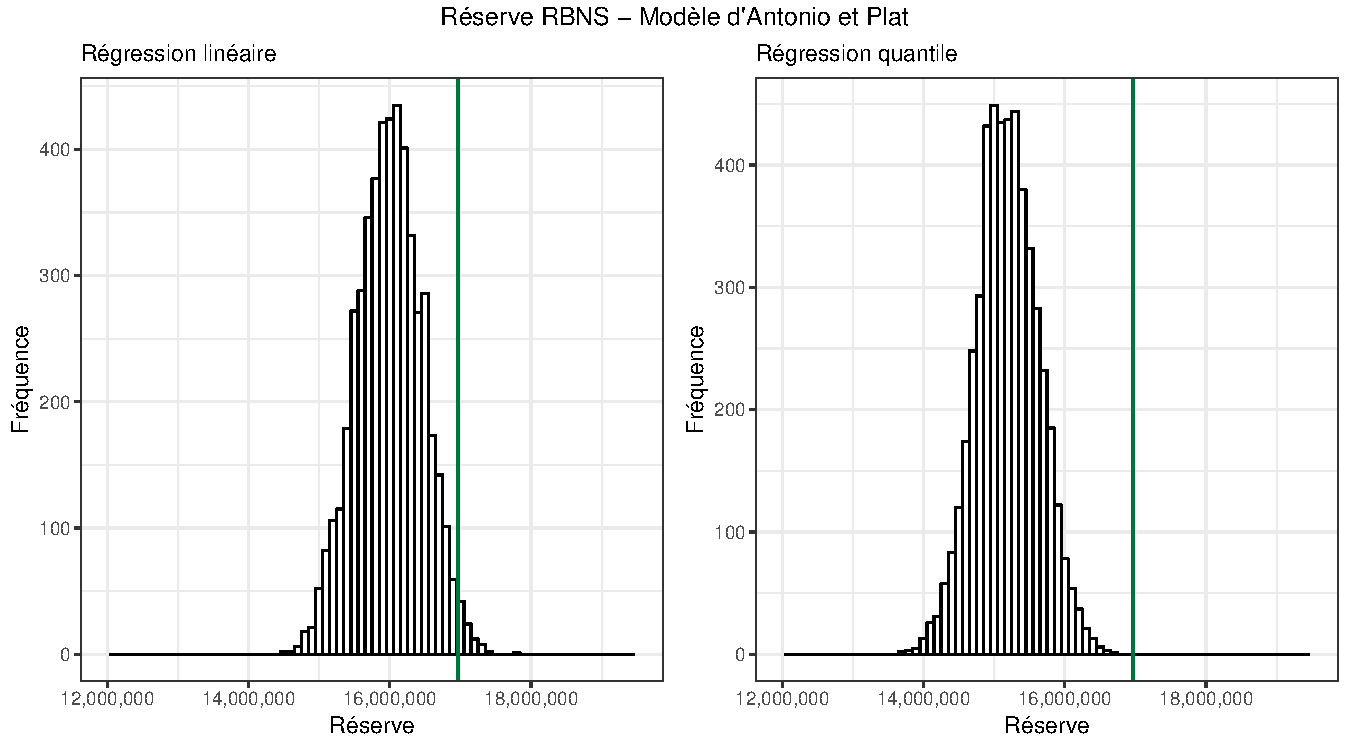
\includegraphics[width = \textwidth]{resultats_reserve_RBNS_01.pdf}
\end{figure}

\begin{itemize}
    \fleche $\texttt{log-paiement} \sim \texttt{DY} + \texttt{DY}^2$
\end{itemize}

\end{frame}

% ----------

\begin{frame}{Résultats - Tous les prédicteurs}

\begin{figure}
    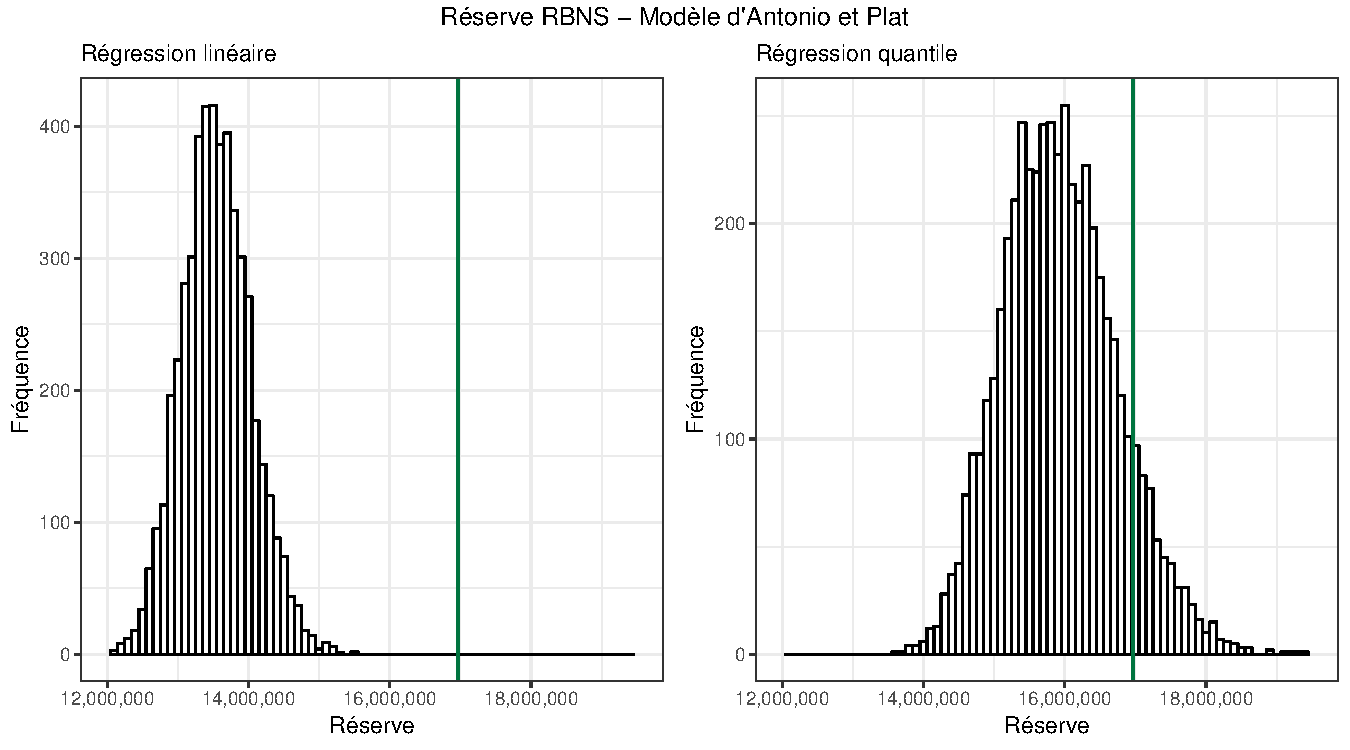
\includegraphics[width = \textwidth]{resultats_reserve_RBNS_02.pdf}
\end{figure}

\begin{itemize}
    \fleche $\texttt{log-paiement} \sim \texttt{DY} + \texttt{DY}^2 + \texttt{AY} + \texttt{RepDel} + \texttt{age} + \texttt{inj\_part}$
\end{itemize}

\end{frame}

% ----------

\begin{frame}{Conclusion}

\begin{itemize}
    \fleche Dans la régression quantile, on devrait utiliser le plus de quantiles possible.
    \fleche L'ajustement de la régression quantile avec modèle linéaire montre qu'on ne peut pas utiliser la régression quantile aveuglément.
    \fleche La statistique de Kolmogorov-Smirnov n'est pas adéquate pour comparer la performance des modèles.
    \fleche Régression quantile pas significativement meilleure que la régression linéaire dans le modèle quadratique selon l'erreur absolue moyenne sur le total.
    \fleche Régression quantile bien meilleure en présence de données aberrantes (lorsque la distribution des paiements est loin d'être lognormale).
    \fleche Régression quantile donne de bons résultats lorsqu'elle est intégrée au modèle d'Antonio et Plat
\end{itemize}

\end{frame}

% ----------

\section{Modifications -- Manuel}
\frame{\sectionpage}
% ----------

\begin{frame}{Mise en contexte}
    \begin{itemize}
            \fleche \textbf{Modèle individuel est très malléable}
            \begin{itemize}
                \cercle Processus de Cox (Avanzi et al, 2016).
                \cercle Ajout de copule (Lopez, 2019).
                \cercle Raccorder une distribution Gamma et une distribution Pareto (Reynkens et al., 2016).
            \end{itemize}
            \pause
            \fleche \textbf{Apprentissage supervisé}
            \begin{itemize}
                \cercle Réseaux de neurones (Kuo, 2018).
                \cercle Gradient boosting (Duval et Pigeon, 2019).
            \end{itemize}
    \end{itemize}
\end{frame}

% ----------

\begin{frame}{Mise en contexte}
    \begin{itemize}
            \fleche \textbf{Arbre de décision (Breiman et al.,1984)}
            \begin{itemize}
                \cercle Modèle individuel non paramétrique entièrement basé sur l’utilisation des arbres de décisions (Wüthrich, 2018).
                \cercle Prendre en considération la censure de la variable prédite (Lopez et al., 2016, 2019).
            \end{itemize}
    \end{itemize}
\end{frame}

\begin{frame}{Mise en contexte}

    \begin{exampleblock}{Question guide}
        Est-ce que l’utilisation d’arbres de décision dans la modélisation des paiements peut être une alternative envisageable à l’approche paramétrique?
    \end{exampleblock}

    \begin{alertblock}{Résumé du projet}
        \begin{itemize}
            \fleche Modélisation de la sévérité des paiements avec les arbres de décisions et des ajustements univarié.
        \end{itemize}
    \end{alertblock}
\end{frame}

\begin{frame}{Conception du modèle}
    \begin{itemize}
        \fleche Arbre de décision pour les paiements.
        \fleche Utiliser la classification faite par la division binaire récursive.
        \fleche Pige aléatoire dans les paiements de la base de données qui respectent chacune des conditions menant à cette feuille.
    \end{itemize}
\end{frame}

\begin{frame}{Conception du modèle}
    \begin{itemize}
        \fleche Règle binaire (continue):
             \begin{align*}
                R_1(b,c) &= \{ X_1 \cdots X_B | X_b \leq c \} \\
                R_2(b,c) &= \{ X_1 \cdots X_B | X_b > c \} \text{ .}
            \end{align*}
    \pause
        \fleche Règle binaire (factorielle):
            \begin{align*}
            R_1(b,c) &= \{ X_1 \cdots X_B | X_b \in c \} \\
            R_2(b,c) &= \{ X_1 \cdots X_B | X_b \notin c \} \text{ .}
            \end{align*}
    \end{itemize}
\end{frame}

\begin{frame}{Conception du modèle}
    \begin{itemize}
        \fleche La fonction objective utilisée est la somme des erreurs au carré (SEC):
             \begin{align*}
    \overline{P} &= \frac{1}{q_{\text{total}}} \sum_{q \geq 1} P_{q} \\
    \text{SEC} &= \sum_{q \geq 1}\left(\overline{P} - P_{q}\right)^{2} \text{,} 
\end{align*}
    \pause
        \fleche Le choix de la covariable $b$ et du $c$ sont ceux qui minimise le SEC suivant:
            \begin{align*}
    \text{SEC} &= \sum_{q \in R_{1}(b,c)}\left(\overline{P}_{R_{1}(b,c)} - P_{q}\right)^{2} + \sum_{q \in R_{2}(b,c)}\left(\overline{P}_{R_{2}(b,c)} - P_{q}\right)^{2} \text{.} 
\end{align*}
    \end{itemize}
\end{frame}
% ----------
% ----------
% ----------
% ----------
% ----------


% ------------------------------------------------------------------------------------------------------------------------------

\end{document}


% \begin{frame}{Processus de Poisson avec marqueurs}

% \begin{itemize}
%     \fleche<1-> On simule d'abord les événements selon le processus de Poisson (ici en 2 dimensions)
%     \fleche<2-> Ensuite on simule le marqueur pour chaque événement
% \end{itemize}

% \begin{figure}
%     \centering
%     \includegraphics<1>[width = 0.6\textwidth]{poisson_process_2d.pdf}
%     \includegraphics<2>[width = 0.6\textwidth]{marked_poisson_process_2d.pdf}
% \end{figure}

% \end{frame}

